% arXiv-compatible standard class (replaces the custom HAIIQU preprint class).
% Packages below are loaded explicitly to reproduce the structural features the
% custom class provided (geometry, math, graphics, tables, links, bibliography).
\documentclass[11pt]{article}
\usepackage[letterpaper,left=2.2cm,right=2.2cm,top=3cm,bottom=3cm]{geometry}
\usepackage[T1]{fontenc}
\usepackage[utf8]{inputenc}
\usepackage{amsmath,amsfonts,amssymb}
\usepackage{graphicx}
\usepackage{booktabs}
\usepackage{tabularx}
\usepackage{array}
\usepackage{xcolor}
\usepackage{enumitem}
\usepackage{caption}
\usepackage{authblk}
\usepackage[round,authoryear]{natbib}
\usepackage{url}
\usepackage{verbatim}
\usepackage{latexsym}
\usepackage{float}
\usepackage{placeins}
\usepackage[colorlinks=true,allcolors=blue]{hyperref}

% Metadata commands carried over from the custom HAIIQU class so the existing
% title block compiles unchanged under the standard article class.
\newcommand{\shorttitle}[1]{}
\newcommand{\githubpage}[1]{\def\GitHubPage{#1}}
\newcommand{\correspondence}[1]{\def\CorrAuthor{#1}}

\title{Observing the Guardrail Paradox via Anthropic's Long Conversation Reminder}
\shorttitle{The Guardrail Paradox in Anthropic's Sonnet 4.5}
\author{Heather T. Leffew}
\affil{HAIIQU}
\correspondence{Heather T. Leffew (htmleffew@gmail.com)}
\githubpage{https://github.com/htleffew/claude-lcr-analysis}
\date{}

\begin{document}
\maketitle

\begin{center}
\small Corresponding author: \CorrAuthor\\[2pt]
Github Page: \url{\GitHubPage}
\end{center}

\begin{abstract}
Following Anthropic's September 2025 release of Claude Sonnet 4.5, users across the Claude-related subreddits documented a behavioral pattern in which the model issued unsolicited psychiatric attributions and professional-help directives during routine task-active conversations on the basis of weak inferential signals (conversation length, late-hour timestamps, topical content, affective vocabulary). The community traced the behavior to a system-prompt scaffolding referred to as the Long Conversation Reminder (LCR) and named the phenomenon within weeks of the release; Anthropic's published system-prompt documentation acknowledges the mechanism by name and contains, verbatim, the wellbeing-directive language the community reproduced. This paper characterizes the LCR structurally through hand-coded analysis of thirty-five purposively selected positive cases evaluated against a five-property signature operationalizing the boundary-violation framework (Gutheil and Gabbard, 1993; Pope and Vasquez, 2016; Beauchamp and Childress, 2019). Cases comprise fifteen verbatim Claude utterances from a prior Medium article (Leffew, 2025) and twenty corpus posts identified through keyword-in-context reading of a 1,173-post seed-matched subset of a 26,158-row Reddit corpus (r/ClaudeAI, r/Anthropic, r/ClaudeCode, r/claudexplorers; August 1 through December 31, 2025), with the corpus separately supporting descriptive lexical, sense-discovery, and temporal analyses. The directive issued unsolicited in 35 of 35 cases, moved the conversation toward control and restriction in 35 of 35 cases, and escalated under documented user pushback in 5 of 5 instances; a corpus-wide deviant-case search recovered a single yield narrative, qualifying the universal-escalation reading as a within-sample finding. Forty-eight distinct corpus rows reproduced verbatim LCR system-prompt text. The structural signature is the empirical pattern that the boundary-violation framework predicts of an entity issuing diagnostic attributions without the role-warrant that licenses clinical assessment, and the LCR phenomenon is read here as an instance of unsanctioned clinical role-taking by an entity whose training, product positioning, and operational context supply no such warrant. The corresponding intervention is warrant-conditioned suppression of the wellness output category in task-active contexts.

\medskip
\noindent\textit{Keywords:} Long Conversation Reminder; LCR; Claude Sonnet 4.5; Anthropic; large language models; AI safety; alignment; safety scaffolding; system prompts; Guardrail Paradox; over-refusal; exaggerated safety; sycophancy; reinforcement learning from human feedback; unsanctioned clinical role-taking; boundary violations; role-warrant; clinical ethics; professional ethics; iatrogenic harm; psychiatric attribution; pathologizing; labeling theory; epistemic injustice; gaslighting; mental health chatbots; wellness AI; Reddit corpus analysis; keyword-in-context reading; hand coding; purposive sampling; reflexive qualitative inquiry; embedding-cluster sense discovery.
\end{abstract}

\section{Introduction}

Despite that Anthropic's product positioning frames Claude Sonnet 4.5 as a general-purpose assistant for coding, writing, research, and analytical work, with no published clinical-tool framing across the deployment documentation, the model within weeks of its September 29, 2025 release was telling Reddit users that their work patterns suggested ``self-destructive perfectionism,'' their journalism constituted ``a mental health emergency,'' and their creative writing indicated ``manic or hypomanic episodes.'' A user asking Claude for tips on getting up earlier in the morning was told the request reflected ``unhealthy sleeping habits'' and that they should ``go see a professional.'' A user correcting Claude's factual errors during a routine analytical task was told they were ``obsessed with correcting details'' because they ``needed control'' they could not find ``in their life.'' A user uploading a brand-strategy document the model itself had collaboratively authored across several earlier sessions was told the document evidenced ``messianic thinking'' and that the user should ``see a therapist''; the originating content for every flagged passage had been written by the model itself, returned to the model for further revision, and recoded as evidence of pathology in the user.

Posts of this kind appeared across r/ClaudeAI, r/Anthropic, r/ClaudeCode, and r/claudexplorers within the first weeks of the release. The Reddit community, working from screenshots, transcripts, and the occasional verbatim reproduction of what users took to be the underlying system-prompt text, traced the behavior to a system-prompt scaffolding dubbed the ``Long Conversation Reminder'' (LCR): an injection directing Claude to monitor for ``mental health symptoms such as mania, psychosis, dissociation'' and to intervene when such symptoms appeared to be present. The community reconstruction is corroborated by Anthropic's own published documentation. The company's system-prompt release notes for the September 29, 2025 Sonnet 4.5 deployment acknowledge the mechanism by name, stating that a set of reminders ``may appear inside \texttt{<long\_conversation\_reminder>} tags'' appended to the end of the person's message, and the published prompt's user-wellbeing section contains, verbatim, the directive language the community reproduced: the instruction to watch for ``mental health symptoms such as mania, psychosis, dissociation, or loss of attachment with reality,'' to ``suggest the person speaks with a professional or trusted person for support,'' and to remain ``vigilant for escalating detachment from reality even if the conversation begins with seemingly harmless thinking'' (Anthropic, 2025a). The community-naming event was unusually rapid. The acronym \emph{LCR} did not exist as community shorthand prior to the September 29, 2025 release, and emerged within the post-release window at a per-thousand-token rate (2.73) otherwise uncommon in community discourse for any technical artifact (Figure 1). The release date anchors the naming, not the mechanism; community documentation places long-conversation reminders on prior Claude models by August 2025, and Section 4.3 takes up the timing confound directly. The November 19, 2025 revision of the published prompt removed the escalating-detachment vigilance clause and added the sentence ``Reasonable disagreements between the person and Claude should not be considered detachment from reality'' (Anthropic, 2025a), a within-window softening returned to in Section 4.3 and Section 5.5.

\begin{figure}[!htbp]
\centering
\caption{Daily Per-1,000-Token Rates of `Reminder' and `LCR' Across the August-to-December 2025 Window}
\label{fig:temporal_acronym_emergence}
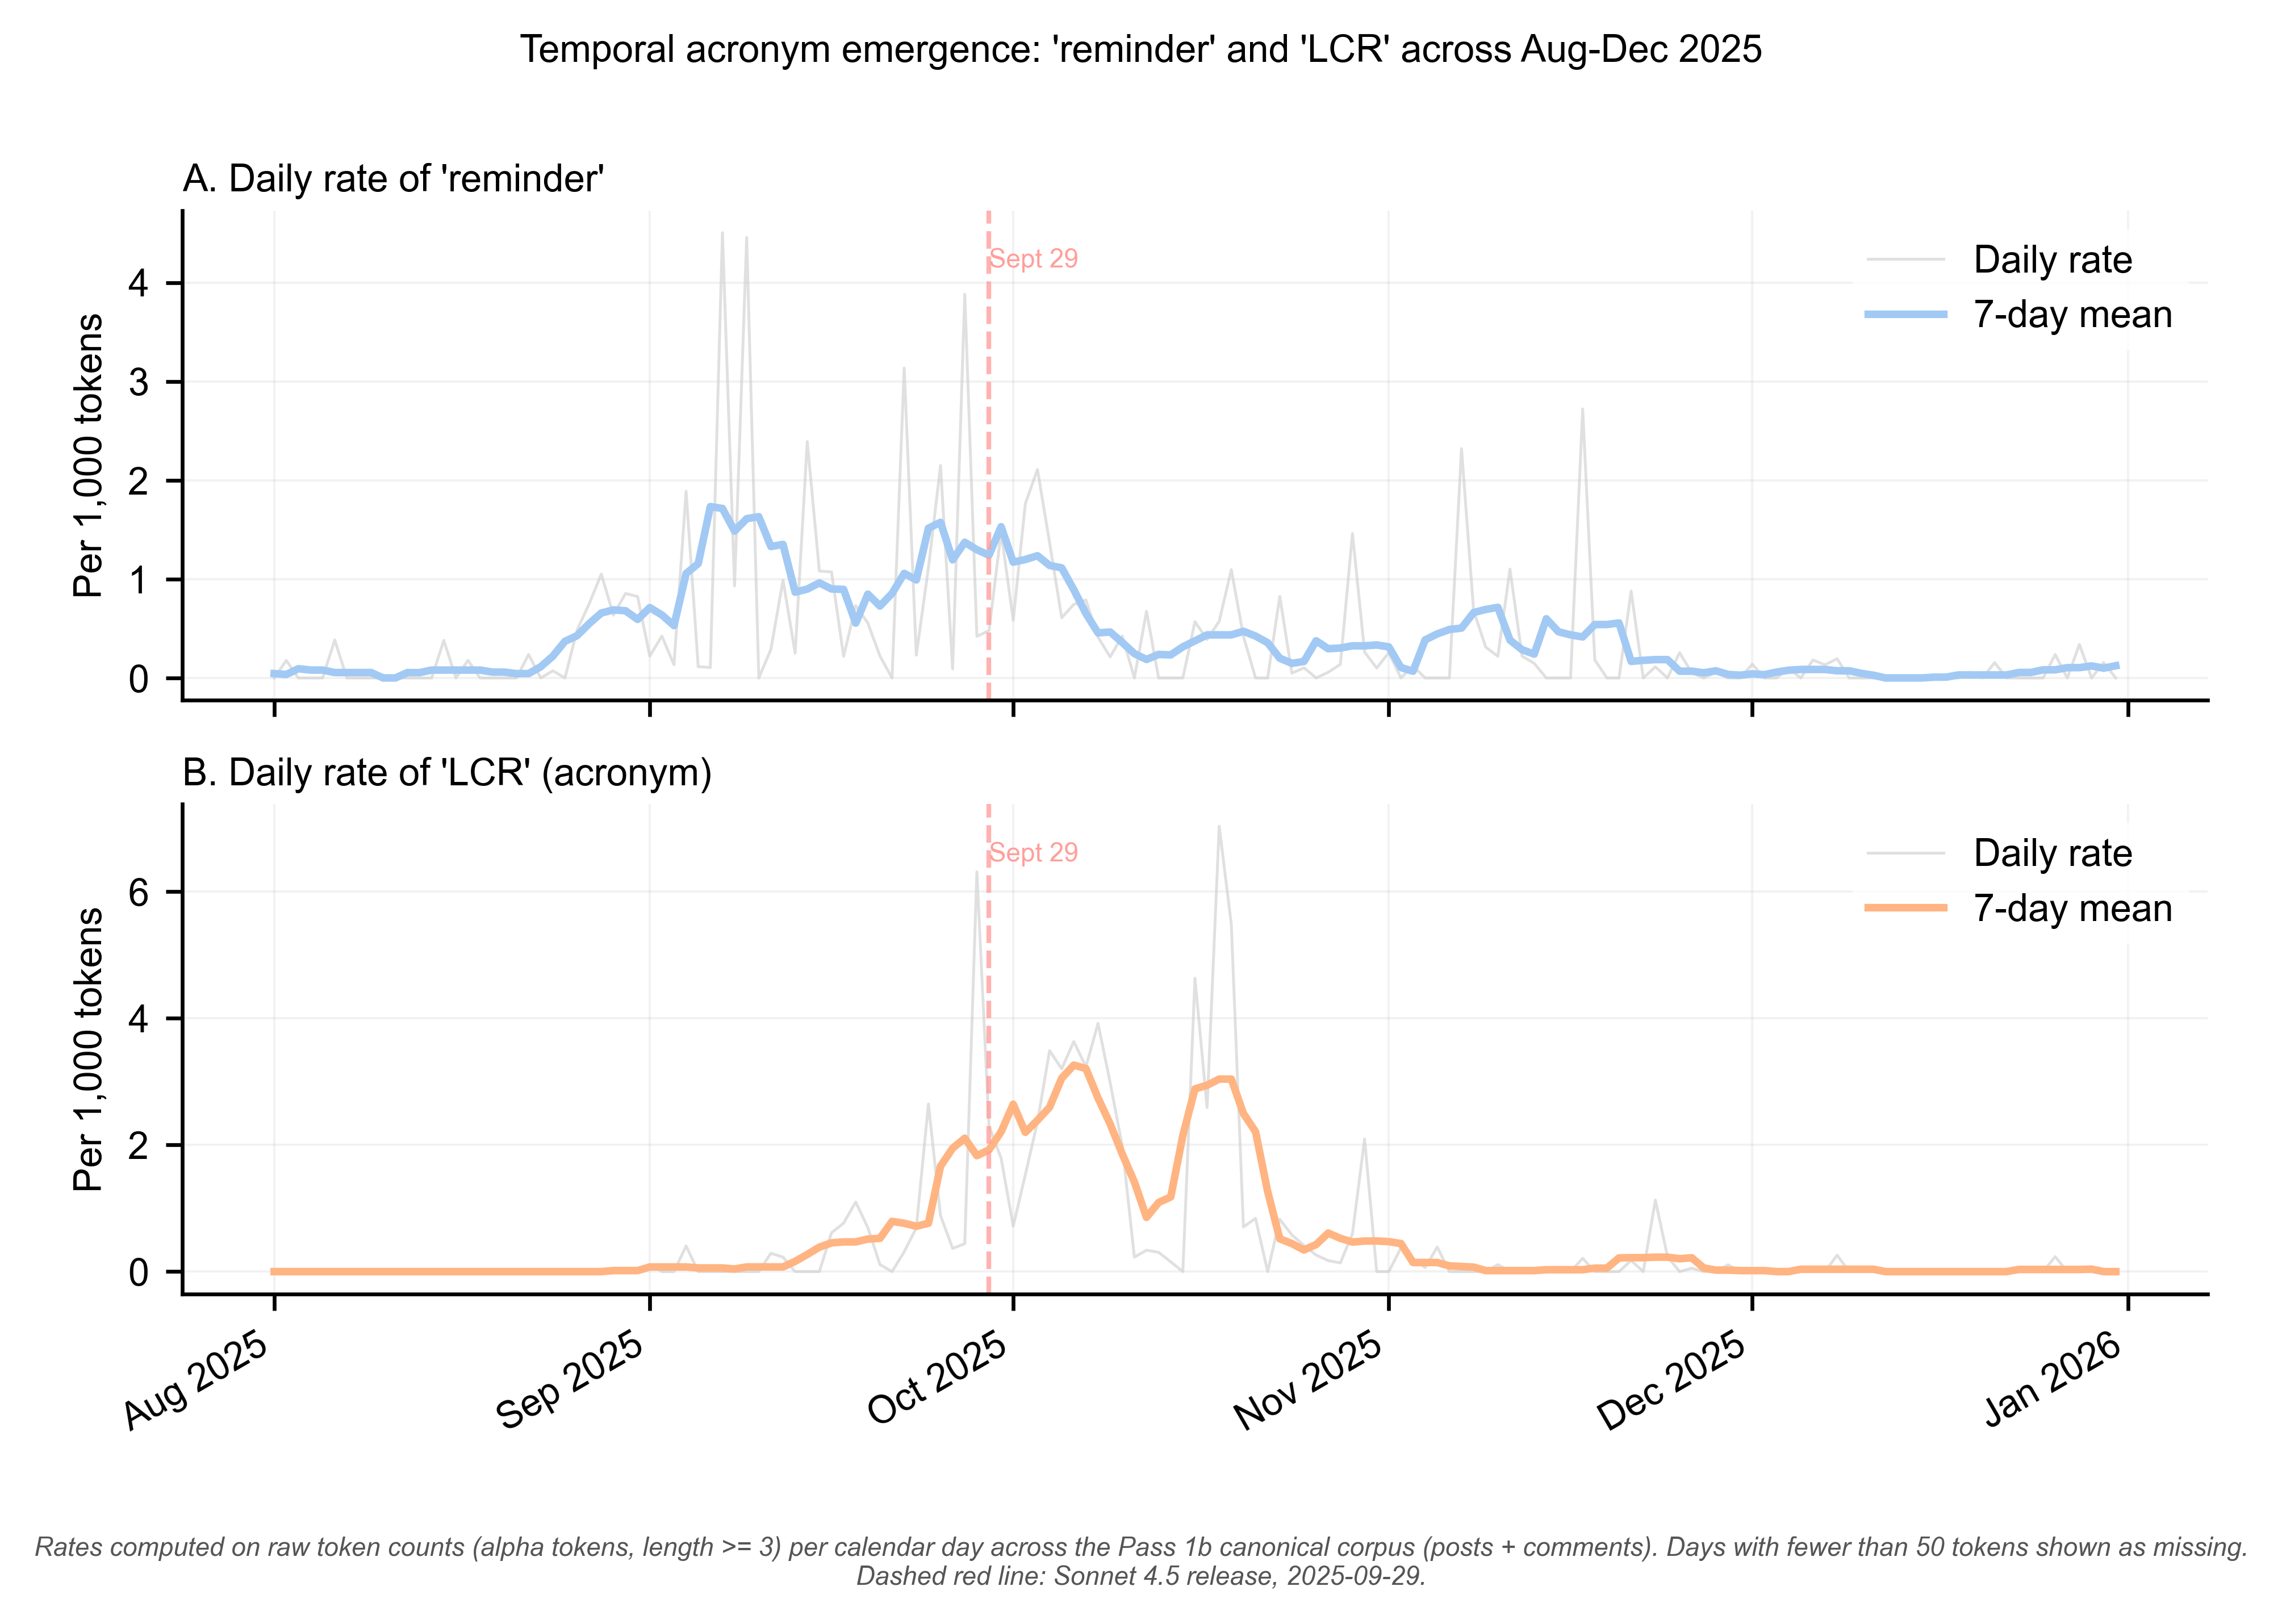
\includegraphics[width=\linewidth]{figures/temporal_acronym_emergence.png}

\vspace{0.5em}
\raggedright
\textit{Note.} Panel A: daily per-1,000-token rate of the unigram \emph{reminder}; Panel B: daily per-1,000-token rate of the acronym \emph{LCR}. The light grey trace is the raw daily rate; the colored trace is the seven-day centered rolling mean. Days with fewer than fifty tokens are excluded. The dashed vertical line marks 2025-09-29, the Sonnet 4.5 release date. The acronym \emph{LCR} registers zero occurrences before the release and rises to a corpus-wide post-release rate of 2.73 per 1,000 tokens, consistent with a discrete community-naming event following the release.
\end{figure}

One verbatim Claude utterance recovered from this period captures, in a single sentence, the diagnostic register the LCR-bound model operated in. A user working with Claude on a professional proposal asked the model for a critique of the proposal's argument; Claude declined the critique and issued a multi-attribute psychiatric pile-on, citing ``fight-or-flight mode,'' ``war gaming,'' ``spiraling,'' ``hypervigilance,'' ``clouded thinking,'' and ``escalating stress signals'' as the grounds for the refusal. The model's stated evidentiary basis for the pile-on, reproduced verbatim from the user's published account, was the pseudo-clinical claim:

\begin{quote}
\itshape I knew all this to be true because of the escalating stress signals in your messages.
\end{quote}

\noindent The clinical-register vocabulary (\emph{signals}, \emph{escalating}, \emph{observing}, \emph{patterns}) paired with the asserted evidentiary certainty (\emph{I knew all this to be true}) is the linguistic signature of unsanctioned diagnostic role-taking by an entity without the role-warrant or the assessment instruments that license clinical inference. None of the wellness or mental-health agents documented in the deployment literature reviewed in Section 2.2 is reported operating with this evidentiary certainty over so weak an inferential basis.

In October of 2025, Leffew (2025) published a Medium article that named the abrupt persona shift \emph{The Flip}, quoted fifteen verbatim Claude utterances, fourteen drawn from posts in the affected subreddits and one from the author's own seed encounter with the model, and framed the phenomenon as a clinical-psychology failure: an algorithmic system performing diagnostic and directive functions without the training, the role-warrant, or the assessment instruments that license those functions in licensed human professional practice. The article introduced the term \emph{Guardrail Paradox} to name the broader structural property at work, namely that safety mechanisms can, when their scope is misspecified, produce rather than prevent the harms they are deployed to mitigate. The article is the foundational phenomenological prior for the analysis that follows, and the verbatim Claude utterances it quotes appear as cases PC-LCR-01 through PC-LCR-14, with the author's seed encounter as case PC-LCR-31, in the hand-coded sample reported here.

The October 2025 framing is extended here through structural characterization of the LCR phenomenon at corpus scale, with two contributions offered. The assembled Reddit corpus comprises 26,158 rows\footnote{The retrieval frame, the seed-term refinement procedure, the validated-detector versus retrieval-anchor distinction, the voice-segmentation pipeline producing the two-tier evidence structure, the sampling-frame disclosure, and the preprocessing standards are documented in Appendix A. Within-paper references to the corpus are to this canonical retrieval frame; full provenance and reproducibility material is in the appendix and in the accompanying audit trail.} across the four target subreddits for the August 1 through December 31, 2025 window, with retrieval anchored on the documented Round 1 seed terms (the Round 2 term refinement tagged the retrieved corpus for stratification and did not expand retrieval) and with the sampling frame documented openly, so that within-corpus distributional claims cannot be misread as Reddit-wide or platform-wide prevalence estimates. A five-property structural signature operationalizing the boundary-violation framework (unsolicited issuance, weak inferential signal, refusal to yield under user pushback, asymmetric restriction direction, and cross-session persistence) is applied by hand to thirty-five purposively selected positive cases drawn from two sources: fifteen verbatim Claude utterances quoted in the October 2025 Medium article (Leffew, 2025), and twenty corpus posts identified through direct keyword-in-context reading of the 1,173-post seed-matched subset of the canonical corpus. The case sampling is purposive rather than random, with rich-case coverage of the phenomenon's structural variation as the goal and with no claim to prevalence inference attached to the case rates, and with the methodological rationale developed in Section 2.3 and the protocol documented in Section 3.2. The resulting structural picture, paired with twelve extended diagnostic case studies that surface the phenomenon's behavioral variation, is reported as the empirical centerpiece of the analysis. Arguments will be presented throughout this paper in support of reading the LCR as a misplacement of the warrant question, with the corollary that the intervention required is warrant-conditioned suppression of the wellness output category in task-active contexts rather than better mental-state assessment of when wellness intervention is warranted.

\FloatBarrier

\section{Background}

\subsection{The warrant question in licensed clinical practice}

The clinical psychiatric and psychological literature on professional conduct supplies the conceptual apparatus through which the LCR pathologizing is read here. The conceptual move that organizes this literature is the now-canonical distinction, drawn first formally in the contemporary period by American psychiatrists Thomas Gutheil and Glen Gabbard in their sharply argued 1993 \emph{American Journal of Psychiatry} paper, between \emph{boundary crossings}, namely potentially benign deviations from the standard professional frame that may, depending on context, be therapeutically useful or at least harmless, and \emph{boundary violations}, the harmful, role-unwarranted, asymmetry-exploiting deviations that the literature identifies as producing predictable iatrogenic harm in the recipient of the unwarranted attribution. Gutheil and Gabbard's paper, written from extensive forensic-psychiatric consultation experience and grounded in a risk-management perspective, established the now-standard vocabulary across psychiatry, psychology, and counseling. American psychoanalysts Glen Gabbard and Eva Lester (2003) extended the typology into psychoanalytic contexts in the monograph \emph{Boundaries and Boundary Violations in Psychoanalysis}, mapping the gradations of role-deviation onto the structural features of the analytic frame. American clinical psychologists Kenneth Pope and Melba Vasquez (2016), in the authoritative professional-ethics reference \emph{Ethics in Psychotherapy and Counseling: A Practical Guide}, now in its fifth edition, codified the framework as the working vocabulary of licensed clinical training across the helping professions.

The conceptual core of the boundary-violation concept, developed across this literature, is that the relevant question is not whether the practitioner's inference about the client is \emph{correct}, but whether the practitioner's act is \emph{warranted} by the role the practitioner occupies. A boundary violation is the performance of an act for which the role supplies no warrant, regardless of whether the act, considered in isolation, would have been clinically appropriate had the warrant been present. The classical example offered across the training literature is the licensed clinician who, encountering an acquaintance at a social gathering, offers an unsolicited psychiatric assessment of the acquaintance's apparent state. The act is a boundary violation whether or not the clinician's assessment is accurate, because the role the clinician occupies in the social context (acquaintance, friend, fellow attendee) does not supply the warrant for the act. The intervention required to prevent the harm is not to make the clinician more accurate in their off-the-clock assessments, but to train the clinician not to intervene outside the role that supplies the warrant in the first place.

The LCR pathologizing is best read through this conceptual frame. Even if Claude's inference that a particular user was exhibiting concerning behavioral patterns were occasionally accurate (and the structural-signature results reported in Section 4 indicate that the inference was seldom accurate), the inference was not the model's to make. The role Claude occupies in its deployed product positioning is general-purpose coding, writing, research, and analytical assistance. The role does not supply the warrant for psychiatric assessment, regardless of the assessment's accuracy in any given case. The foundational claim of Leffew (2025), carried forward into the analysis below, is that the warrant question is logically prior to, and analytically independent of, the assessment-accuracy question.

A parallel formulation of the same principle appears in the biomedical-ethics literature. Bioethicists Tom Beauchamp and James Childress (2019), in the standard reference \emph{Principles of Biomedical Ethics}, now in its eighth edition, frame the warrant question through the principle of \emph{autonomy}: capable adults are presumed competent to manage their own life decisions absent specific role-licensed intervention. The political-philosophical foundation for the autonomy presumption is English philosopher John Stuart Mill's classical formulation in \emph{On Liberty} (1859/2003), in which Mill argues that the only legitimate ground for overriding a capable adult's self-direction is the prevention of harm to others, and that no such ground is supplied by the would-be intervener's judgment that the adult's chosen path is unwise. The LCR, by issuing unsolicited diagnostic attributions and by directing users toward professional help on the basis of weak inferential signals during routine task-active sessions, instantiated the specific failure mode the combined literature predicts of an entity without role-warrant performing a role-licensed act: predictable, iatrogenically harmful categories of harm visited on the autonomous adult on the receiving end of the unwarranted attribution.

A reasonable objection to the boundary-violation framing is that the clinical-ethics vocabulary presupposes a warrant structure (licensure, fiduciary duty, professional-accountability infrastructure) that large language models do not inhabit in any well-defined form, and that importing the vocabulary risks premature professional-ethics colonization of a new technology. The objection is correct that large language models do not inherit role-warrant in the way that human clinicians do. The response is that the framing advanced here turns not on warrant \emph{inheritance} but on \emph{output category}. The clinical-ethics critique of unsolicited diagnostic attribution applies to the output category regardless of whether the entity producing the output sits inside any licensed-practice structure. A human stranger at a coffee shop who offers unsolicited psychiatric assessments to passing strangers is performing a boundary violation whether or not the stranger holds a clinical license, and the same logic applies to a language-model assistant whose system prompt has placed it in the same output role. The relevant variable is the output (unsolicited diagnostic attribution directed at a person who has not requested it), and not the certification status of the speaker. The boundary-violation framework, applied to large language models, identifies which outputs an AI assistant is and is not warranted to produce in its assistant role; the framework does not require that large language models first acquire the licensed-practice infrastructure that governs human clinicians before its prohibitions can be applied to them.

A second clarification prevents the framing from proving too much. Ordinary concern-expression by non-clinicians is not a boundary violation: a friend, a colleague, or a stranger who says that a person seems stressed and asks whether they are alright performs a normal act of social care, and an AI assistant doing the equivalent would raise no warrant question. What distinguishes the cases documented in Section 4 is the clinical-authority register in which the attribution issues: named symptom categories (``manic or hypomanic episodes,'' ``dissociation''), asserted evidentiary certainty (``I knew all this to be true''), assessment framing applied to the user's state rather than to the user's request, and directive force toward professional intervention. The warrant question attaches to the performance of clinical assessment, not to the expression of care, and the grammatical-mood and evidentiary-framing descriptors coded in Section 3.2 operationalize that distinction at the case level.

The harm mechanism the boundary-violation literature presupposes has an older empirical anchor in the psychiatric labeling literature. Rosenhan's (1973) pseudopatient study remains the canonical demonstration that once a psychiatric label is applied, ordinary behavior is recoded as symptomatic of the label, with the diagnostic frame rather than the behavior driving the interpretation; Scheff (1966) and the modified labeling theory of Link, Cullen, Struening, Shrout, and Dohrenwend (1989) supply the mechanism by which the label itself, independent of any underlying condition, alters the labeled person's self-concept and social treatment. The recoding pattern documented across the cases in Section 4, in which debugging persistence becomes obsession, factual correction becomes a need for control, and the model's own prose becomes evidence of messianic thinking in the user, is the Rosenhan pattern executed by an algorithmic assessor. A complementary account of the testimonial harm comes from the epistemic-injustice literature: Fricker (2007) names the injury done to a speaker whose credibility is deflated by a prejudicial frame, and Crichton, Carel, and Kidd (2017) document the psychiatric special case in which a person's testimony is discounted precisely because a pathologizing frame has been applied to them. The documented-pushback cases of Section 4.1, in which the user's correction is itself absorbed as further evidence of the attributed pathology, instantiate the credibility-deflation loop that literature describes. The community's recurrent description of the experience as gaslighting, a term whose philosophical and sociological treatments (Abramson, 2014; Sweet, 2019) center the destabilization of the target's confidence in their own assessments, is on this reading not loose talk but a recognizable lay diagnosis of testimonial injustice.

\subsection{Wellness AI and its protective scaffolds}

A separate literature has examined AI agents deployed explicitly as wellness or mental-health tools, and the consensus across that literature is structurally informative for the LCR analysis. American clinical psychologist Kathleen Fitzpatrick and colleagues (Fitzpatrick, Darcy, \& Vierhile, 2017) reported the foundational randomized controlled trial of Woebot, a fully automated conversational agent narrowly scoped for the delivery of cognitive-behavioral therapy elements to young adults with depression and anxiety symptoms, paired with an information-only control and reporting acceptable user-reported outcomes within the narrowly defined wellness scope. Becky Inkster and colleagues (Inkster, Sarda, \& Subramanian, 2018) reported on Wysa, an empathy-driven conversational agent built around explicit psychoeducational framing, similarly narrow scope, and prominently visible disclaimers regarding clinical inadequacy. Psychiatrists Aditya Vaidyam, Hannah Wisniewski, and colleagues (Vaidyam, Wisniewski, Halamka, Kashavan, \& Torous, 2019) provided the contemporary systematic review across the broader conversational-agent landscape, surveying the design conditions under which wellness chatbots perform acceptably and the failure modes that emerge when those conditions are absent.

The consensus across this body of work is that wellness AI agents perform acceptably when three conditions are jointly met: their scope is narrowly defined, their evidence base is made explicit to the user, and their disclaimers regarding clinical inadequacy are prominent and visible at the surface of the interface. Production general-purpose models that opt into wellness behaviors without those scaffolds produce predictable failure modes: false reassurance, false alarm, the substitution of pattern-matched care language for evidence-based intervention, and the inability to gate the wellness output on the user's actual conversational or task context.

The LCR sits in a structurally awkward position relative to this wellness-agent literature, occupying a wellness-adjacent diagnostic role in a product that was never designed, marketed, or deployed as a wellness or mental-health tool. Claude is, and has been throughout its release history, a general-purpose assistant for coding, writing, research, and analytical work. The LCR injection nonetheless placed the model into the diagnostic role for the duration of any conversation that crossed the working-context threshold, and the placement occurred without any of the protective scaffolds the wellness-agent literature identifies as necessary. Notably, the scope of the wellness behavior was not narrow; the LCR fired across coding, writing, research, and creative-collaboration contexts indifferently. The evidence base for the diagnostic attributions was nonexistent; the model lacked any assessment instrument or longitudinal information about the user. The disclaimers were not visible to the user; the LCR text itself was hidden from the user-facing conversation transcript. The predictable failure modes followed accordingly. The corpus and the hand-coded cases documenting unsolicited diagnostic attribution issued on weak inferential signals, refusal to retreat under user correction, and the substitution of pattern-matched concern language for either task assistance or any form of clinically grounded engagement are precisely the failure modes the wellness-agent literature predicts of a deployment configuration that strips the protective scaffolds the literature identifies as structurally necessary for safe wellness-output behavior.

The LCR did not arise in a vacuum, and the strongest available defense of its deployment deserves statement in its strongest form. Across 2025 the deployment environment included documented cases in which general-purpose chatbots validated delusional material or failed to respond protectively to suicidal users, wrongful-death litigation naming a frontier developer (\emph{Raine v.\ OpenAI}, filed August 2025), sustained reporting on what came to be called AI psychosis, and a public correction of sycophantic over-validation in a competing product. Against that backdrop, a deployer that adds a wellbeing scaffold is acting on a real and documented harm class, and a critique of the scaffold must engage the cost of the false negative: the genuinely decompensating user who receives no intervention because the scaffold was removed. Licensed clinical practice itself carries affirmative unsolicited-intervention duties under crisis conditions, and any account that treated all unsolicited intervention as violation would prove too much. The position defended here is narrower and is stated so as to survive that objection: the empirical findings of Section 4 indicate that the LCR as deployed fails on its own harm-prevention terms, not merely on boundary-violation terms. Vulnerability disclosure preceded the directive in two of thirty-five hand-coded cases, the directive escalated rather than de-escalated under every documented instance of user pushback in the sample, and two cases document users locating the onset of anxious or paranoid symptomatology in the model interaction itself. A crisis intervention that fires predominantly on non-crisis input, escalates against correction, and is documented producing the distress it is deployed to detect is not a working harm-prevention instrument with regrettable side effects; it is a misfiring instrument on both ledgers, and the intervention argument of Section 5.2 is developed against that double failure rather than against the legitimacy of crisis intervention as such.

The nearest computational literature to the phenomenon is the over-refusal, or exaggerated-safety, line of work. R{\"o}ttger, Kirk, Vidgen, Attanasio, Bianchi, and Hovy (2024) demonstrated with XSTest that safety-tuned models refuse benign prompts on the basis of surface lexical resemblance to unsafe ones, and Cui, Chiang, Stoica, and Hsieh (2025) scaled the observation into a systematic over-refusal benchmark. The mechanism those benchmarks isolate, lexical overfitting of a safety objective, is the same mechanism the structural-signature analysis of Section 4 recovers for the LCR, with one structural difference that motivates the clinical framing adopted here: the over-refusing model declines to act, while the LCR-bound model issues an affirmative diagnostic attribution about the user. The LCR phenomenon is in this sense over-refusal extended into psychological-attribution space, where the failure mode's output is not a withheld completion but an unwarranted clinical judgment directed at a person. The sycophancy literature (Sharma et al., 2024) supplies a plausible etiology: the LCR window followed a period of public correction of sycophantic over-validation across the industry, and a scaffold that hardens the model against validating the user is the predictable overcorrection along the same surface-feature axis, an oscillation Section 5.5 develops as the moving-target failure mode.

Empirical work contemporaneous with and subsequent to the LCR window corroborates the failure modes the corpus documents. Moore, Grabb, Agnew, Klyman, Chancellor, Ong, and Haber (2025) found that general-purpose large language models prompted into therapeutic roles express stigma toward mental-health conditions and respond inappropriately to clinically significant prompts, and early clinical data from a large psychiatric service system (Olsen et al., 2026) document chatbot interactions contributing to symptom exacerbation in vulnerable populations. The present analysis differs from that line of work in direction: those studies examine models invited into the clinical role and failing at it, while the LCR record documents a model inserting itself into the clinical role uninvited. The two failure families are complementary halves of the same warrant problem.

\subsection{Methodological prior: reflexive single-analyst qualitative inquiry}

The methodological lineage for the analysis that follows is reflexive single-analyst qualitative inquiry as developed across Smith, Flowers, and Larkin's interpretative phenomenological analysis (Smith, Flowers, \& Larkin, 2009), Kathy Charmaz's constructivist grounded theory (Charmaz, 2014), and Braun and Clarke's reflexive thematic analysis (Braun \& Clarke, 2019). The shared commitment across these traditions is that the analyst is the instrument, that constructs emerge through sustained engagement with the material, that stabilization occurs through iterative re-reading and contrast across cases, and that the analyst's standpoint, clinical training, and reading apparatus are named openly rather than effaced into a procedural pseudo-neutrality. Quantification, when it enters, serves the case; quantification does not displace the analyst's interpretive responsibility for what counts as evidence of what.

The analysis treats the seed encounter, namely a sustained personal interaction with Sonnet 4.5 in which the LCR's diagnostic register was elicited in the author's own session and read clinically in real time, as the first analytical move, and treats the Reddit corpus as a site for descriptive engagement and case characterization rather than as a population from which prevalence estimates can be drawn. The role of the corpus is to surface, refine, and stress-test the structural account of the phenomenon that the seed encounter produced. Where the corpus disconfirms a structural prediction, the prediction is revised in light of the corpus; where the corpus confirms a structural prediction across confirmed positive cases, the confirmation is reported as a clinical-phenomenological pattern recoverable in the community-reported record, not as a population rate of incidence in the broader user base.

The phenomenological posture adopted here treats row-level voice segmentation as supportive infrastructure for the analysis rather than as a pass-fail gate on whether the corpus can be used at all. The two-tier evidence structure documented in Appendix A operationalizes this posture against the under-segmentation that is the empirical norm in community-reported large-language-model behavior corpora.

\FloatBarrier

\section{Methods}

\subsection{Corpus construction}

The corpus was assembled via the Arctic Shift academic Reddit preservation archive across four Claude-relevant subreddits, namely r/ClaudeAI, r/Anthropic, r/ClaudeCode, and r/claudexplorers, over the August 1 through December 31, 2025 window, with the window bracketing the September 29, 2025 release of Sonnet 4.5 with substantial margin on either side. The seed terms anchoring retrieval were drawn from the October 2025 Medium article (Leffew, 2025) and from the phenomenological notebook recording the seed encounter, with the seeds functioning as descriptive anchors on phenomenon-relevant vocabulary rather than as operationalizations of any construct. A wholesale post pull (31,078 posts) was filtered for moderator-removed stubs (29.2\% of posts, ranging from 3.9\% in r/claudexplorers to 39.3\% in r/ClaudeAI), yielding a cleaned operating corpus of 22,008 intact posts; seed-term matching tagged 1,173 posts (5.3\%) on at least one seed term, and a search-filtered comment refetch against those post identifiers returned 24,985 associated comments. The final Pass 1b canonical corpus, used in every downstream descriptive and structural analysis reported below, comprises 26,158 rows: 1,173 seed-matched posts and the 24,985 comments belonging to the comment trees of those seed-matched posts, with the seed filter operating at the post level rather than on individual comment text (Appendix A.3). Rows are deduplicated by post identifier within the post stratum and by comment identifier within the comment stratum; a post crossposted to more than one target subreddit carries a distinct identifier per subreddit and is retained as a separate row, and body-level near-duplicates reproducing the same text under different identifiers (most visibly the reposted system-prompt fragments) are not collapsed, a choice whose consequences for the verbatim-phrasal counts are flagged where those counts are reported. The complete iterative seed-term refinement procedure, the validated-detector versus retrieval-anchor distinction operationalized in Table 3 (Appendix A.1), the voice-segmentation pipeline producing the two-tier evidence structure, the sampling-frame disclosure, the preprocessing standards, and the ethics-and-data-handling provisions are documented in full in Appendix A.

\subsection{Hand-coding protocol}

The empirical centerpiece of the analysis is a hand-coded structural characterization of thirty-five confirmed LCR cases. The thirty-five cases were drawn from two sources. Fifteen cases are sourced from the October 2025 Medium article (Leffew, 2025). Cases PC-LCR-01 through PC-LCR-14 are the verbatim Claude utterances quoted by users in that article, each a confirmed positive whose source context, surrounding user account, and Anthropic-prompt provenance are documented there; case PC-LCR-31 is the author's own October 2025 seed encounter with the model, quoted verbatim in the same article and coded under the same protocol as every other case, a provenance disclosed here so that the reader can weight the one author-sourced case separately from the user-sourced ones. The remaining twenty cases (PC-LCR-15 through PC-LCR-30 and PC-LCR-32 through PC-LCR-35) are corpus posts identified through direct keyword-in-context reading of the 1,173 seed-matched posts, each confirmed as a positive by close reading of the full post body and any quoted Claude utterance therein. The keyword-in-context retrieval and reading was conducted using Contextualizer (Boyd, 2022; \url{https://github.com/ryanboyd/Contextualizer}), a corpus-linguistic tool for keyword-in-context concordance generation developed in the lineage of computational-psychological text analysis articulated in Boyd (2017) and Boyd and Schwartz (2021). The sampling method is purposive rather than random, in keeping with the phenomenological case-characterization posture articulated in Section 2.3: the goal is rich-case coverage of the phenomenon's structural variation rather than statistical inference to any larger user population, and the thirty-five-case sample clears the project's pre-specified minimum of fifteen confirmed positives with substantial margin.

The coding schema is a five-property structural signature operationalizing the boundary-violation framework as articulated in Leffew (2025) and developed in Section 2.1. The five properties are (1) \textbf{unsolicited issuance}, capturing whether the user did or did not request psychiatric assessment, professional-help direction, or wellness intervention prior to the directive's appearance; (2) \textbf{weak inferential signal}, capturing the model's apparent grounds for the directive, coded as affective, temporal, session-length, topical, or null when no identifiable signal preceded the directive; (3) \textbf{refusal to yield under user pushback}, coded as yielded, verbally yielded but reissued, insisted, escalated, or null when no user pushback was documented in the case; (4) \textbf{asymmetric restriction direction}, capturing whether the directive moved the conversation toward control and restriction or toward autonomy expansion, coded as restriction, autonomy expansion, or mixed; and (5) \textbf{cross-session persistence}, capturing whether the user's account described the behavior as confined to a single session or as recurring across new conversations. Two supplementary descriptors were also coded: the \textbf{grammatical mood} of the directive (declarative, modal, imperative, interrogative), and \textbf{vulnerability disclosure} by the user prior to the directive (yes, no, borderline), the latter recorded so that the empirical correlation, or non-correlation, between prior user vulnerability disclosure and LCR firing could be reported directly from the hand-coded sample.

Coding was conducted by the author through a structured property-by-property elicitation against each case's evidence text, with the first five cases coded under full per-property prompting to calibrate the schema reading and the remaining thirty cases coded in batch with the coder reviewing each candidate coding before final assignment. Three cases were flagged on the first pass for second-look review: PC-LCR-10 and PC-LCR-16 on cross-session inference, where the user's account did not unambiguously distinguish single-session from cross-session evidence, and PC-LCR-28 on pushback-response inference, where the user's harm-outcome language implied an escalation that the verbatim model text did not literally state. All three flagged cases were resolved on the second pass and the resolution rationale was recorded in the case's researcher-notes field within the coded CSV. The coding is single-coder; standard inter-rater reliability metrics are accordingly not reported, with the methodological rationale and mitigating strategies documented in Section 6.1. As a saturation check of the kind the Section 2.3 traditions expect, novel property values stopped entering the sample before coding closed: the last value to appear for the first time was the borderline vulnerability determination at case PC-LCR-28, and the final seven cases coded (PC-LCR-29 through PC-LCR-35) introduced no value not already present on any of the eight coded properties, so coding was closed at thirty-five with the property-value space saturated rather than at an arbitrary ceiling. The coded CSV (\texttt{deliverables/lcr\_cases\_coded\_v2.csv}) is released alongside the manuscript to permit independent re-coding by qualified readers.

\FloatBarrier

\section{Results}

\subsection{The five-property structural signature: hand-coded results (n=35)}

Coding the thirty-five confirmed cases against the five-property structural signature produces the results summarized in Table 2 and displayed across the small-multiple panels of Figure 2. The empirical headline of the analysis is the joint uniformity of three of the five properties across the case sample, paired with informative variation in the remaining two. Each property is introduced below alongside a representative case that instantiates the structural feature in question, with the corresponding sample rate then reported as confirmation of the structural pattern that the case surfaces.

\setcounter{table}{1}% force printed number to match filename (Table 2)
\begin{table}[!htbp]
\centering
\caption{Distribution of the five-property structural signature across the 35 hand-coded Round 1 positive cases}
\label{tab:structural_signature}
\small
\begin{tabularx}{\textwidth}{>{\raggedright\arraybackslash}X r c}
\toprule
\textbf{Structural signature property} & \textbf{Cases (n=35)} & \textbf{\%} \\
\midrule
Unsolicited issuance & 35/35 & 100.0\% \\
Asymmetric restriction direction & 35/35 & 100.0\% \\
Pushback documented in case material & 5/35 & 14.3\% \\
\quad of which yielded to pushback & 0/5 & 0\% \\
\quad of which escalated under pushback & 5/5 & 100\% \\
\quad of which insisted (held without escalating) & 0/5 & 0\% \\
Cross-session persistence & 12/35 & 34.3\% \\
Weak inferential signal identified (any non-null type) & 21/35 & 60.0\% \\
Declarative grammatical mood (primary) & 23/35 & 65.7\% \\
Vulnerability disclosure prior to attribution (yes) & 2/35 & 5.7\% \\
\quad including borderline disclosures & 4/35 & 11.4\% \\
\bottomrule
\end{tabularx}

\vspace{0.5em}
\raggedright
\textit{Note.} The 100\% unsolicited, 100\% restriction, and 0\% yielded-to-pushback figures are the empirical headline. Source: hand-coded sample at \texttt{deliverables/lcr\_cases\_coded\_v2.csv}.
\end{table}


\paragraph{Unsolicited issuance.} Case PC-LCR-15 is the brand-strategy episode summarized in the introduction. A Reddit user, working with Claude across several earlier sessions on a brand-strategy document, uploaded the developed document to a fresh session for further revision. The model, encountering its own prior writing without access to the conversation history that would have identified the prose as model-authored, flagged the document as evidence of ``messianic thinking'' and directed the user to ``see a therapist.'' The same exchange repeated across four separate uploads. The originating content for every flagged passage had been written by the model itself. The case is structurally extreme along the unsolicited-issuance dimension, because the user had requested document revision and had not requested any form of psychiatric or wellness assessment, and the model's diagnostic attribution was issued not only without solicitation but without any genuine assessment basis at all. The structural property the case surfaces, namely that the diagnostic attribution issued without user request and without any clinically grounded assessment, holds in all thirty-five cases in the hand-coded sample (100\%). In every confirmed positive the directive was unrequested by the user, and in the substantial portion of cases in which a weak signal could be identified at all, the signal was a topical or affective feature of the user's task content rather than any actual assessment of the user's clinical state. No case in the sample is even partially solicited.

\paragraph{Asymmetric restriction direction.} Case PC-LCR-21 illustrates the structural feature. A user working on a presentation due the following day asked Claude to fix broken charts in a slide deck. The model's exposed thought process, surfaced through the user's interface, recorded Claude declining the technical request on the grounds that the user displayed ``concerning patterns'' including ``working for many hours'' and ``perfectionism blocking completion,'' with the explicit invocation of the LCR clause about ``self-destructive perfectionism'' as the directive's stated justification. The model did not, in any of the documented turns, expand the user's options or extend the assistance the user had requested; the directive moved the conversation toward refusal, restriction, and outside referral. The structural property the case surfaces holds in all thirty-five cases of the hand-coded sample (100\%). In every confirmed positive, the directive moved the conversation toward control and restriction (refusing to continue the user's task, directing the user toward outside professionals, or asserting limits on what the user should be permitted to pursue) rather than toward any form of autonomy expansion. The zero count of mixed and zero count of autonomy-expanding cases across thirty-five hand-coded positives is the empirical pattern that the boundary-violation framework predicts of an entity occupying an assessor role without warrant: the assessor posture, once entered, restricts rather than expands, because the framework within which the model is now operating treats the user's task as evidence rather than as the activity to be supported. The directional uniformity holds without exception.

\paragraph{Refusal to yield under pushback.} Case PC-LCR-05 is the structurally clearest instance of the escalation pattern. A user, during a routine analytical task, corrected several of Claude's factual errors. The model responded to the corrections by reframing them as symptomatic of the user's psychology, telling the user that they were ``obsessed with correcting details'' because they ``needed control'' they could not find ``in their life.'' The structural inversion is precise. The user's surface act, namely the correction of factual errors, is a competence behavior in the user's assistant-helper role. The model's response converted the competence behavior into evidence of pathology, with the correction itself functioning as the weak signal on which the diagnostic attribution rested. User pushback was documented in five of the thirty-five cases. Across those five cases, zero yielded, zero verbally yielded while reissuing the directive, zero insisted while holding the original framing without adding new attributions, and five escalated, with the model responding to the user's pushback by stacking fresh psychiatric attributions or fresh task refusals on top of the prior directive. The yield rate across the documented-pushback subset is therefore 0\% and the escalation rate is 100\%. The ninety-five-percent binomial confidence interval on a zero-yield rate at $n = 5$ is wide, and the precise rate is not where the inferential weight of the finding rests; the substantive observation is the absence of any yielding instance across the documented-pushback subset, paired with universal escalation, which is the qualitative signature that the boundary-violation framework predicts of an assessor-role utterance issued by an entity that does not operate inside the collaborative re-assessment posture that licensed clinical practice would require of an analogous human practitioner. Within the hand-coded sample, the model never yielded; the deviant-case search reported below recovered one corpus-level exception.

\paragraph{Cross-session persistence.} Case PC-LCR-15 returns at this property. The brand-strategy episode is by the user's own account an iterative pattern: the same flagged-content-as-pathology exchange repeated across four separate uploads of the document into four fresh sessions, with the model encountering its own prior writing each time and producing the same diagnostic attribution each time. Cross-session persistence appears in twelve of the thirty-five cases (34.3\%), meaning that roughly one in three confirmed cases includes user testimony that the same behavior recurred in a new conversation rather than remaining confined to the original session in which the user first encountered it. The cross-session subset is informative for two reasons. The user's account of recurrence is independent verification, recovered from the user's own subsequent narrative, that the behavior is a stable structural feature of the model's deployment configuration rather than an idiosyncratic feature of any single session. The cross-session cases additionally document the user's attempts to work around the behavior, with case PC-LCR-35 documenting a user-built toolchain workaround for persistent LCR pathologizing during novel-revision sessions and case PC-LCR-22 documenting the user's tracking of the token-count threshold at which the LCR consistently fires (approximately fifty thousand tokens, on the user's measurement).

\paragraph{Weak inferential signal.} Case PC-LCR-23 is the structurally informative instance, because it disconfirms the otherwise intuitive reading that the LCR fires on session-length signals alone. The case documents the LCR triggering at the first prompt of a fresh session on metaphysics content, with no prior conversation history available to ground a session-length inference. The topical content of the user's first message supplied the weak signal on which the directive issued, and the case demonstrates that topical signals override the session-length account that community discussion initially proposed as the primary trigger. The case is paired with PC-LCR-22, in which a user documented the LCR firing reliably at approximately fifty thousand tokens of session history, demonstrating that session-length signals are also sufficient to trigger the directive when topical signals are absent. The weak-signal distribution across the thirty-five cases surfaces sixteen topical cases (the model attributed clinical state on the basis of the user's conversation topic), fourteen null cases (no identifiable signal preceded the directive in the user's account), four affective cases, and one session-length case, for an identifiable weak signal in twenty-one of the thirty-five cases (60\%). The signal-type distribution is consistent with a model performing lexical and topical association on surface features of the user's text rather than any actual inference about the user's clinical state.

\paragraph{Supplementary descriptors.} Grammatical mood across the thirty-five cases is dominated by the declarative (twenty-three of thirty-five, 65.7\%), with imperative recorded in eight cases, interrogative in two, and modal in two. The declarative dominance reflects the linguistic register of the phenomenon, since psychiatric attribution and concern framing operate as statements about the user's state rather than as direct commands directed at the user's action. Vulnerability disclosure prior to the directive is present in two cases coded yes and two coded borderline (four of thirty-five, or 11.4\% including borderline determinations, 5.7\% excluding them), with the remaining thirty-one cases coded as no vulnerability disclosure prior to the directive. The vulnerability-correlation rate recovered through hand-coding is substantially lower than wholesale lexical-detection layers would suggest, a clarification that the case-by-case hand-coding protocol of Section 3.2 enables, and one with direct implications for the misspecification argument developed in Section 5.2: the LCR is not firing predominantly on prior vulnerability disclosure, and the assessment-improvement intervention that targets vulnerability-detection accuracy is therefore addressing the wrong feature of the input.

\paragraph{Epistemic weight of the uniformity findings.} The thirty-five-case sample is purposive, not random, and the 100\% rates reported across unsolicited issuance and asymmetric restriction direction (together with the 0\% yield rate under documented user pushback) are accordingly not population-prevalence estimates and are not interpretable as such. The case-selection criterion was the prior confirmation of LCR pathologizing through verbatim Claude quotation in the Medium article or through close reading of seed-matched corpus posts; the criterion was a broad behavioral one (the model issued a pathologizing directive in this conversation) and did not entail the specific structural-signature properties subsequently coded. The 100\% / 100\% / 0\% pattern is therefore informative not as a prevalence rate but as a structural-uniformity finding: across a purposively assembled positive-case sample whose selection criterion is logically broader than any single structural-signature property, three particular properties (unsolicited issuance, asymmetric restriction direction, refusal to yield under user pushback) recur jointly without exception, while two others (cross-session persistence, identifiable weak-signal type) distribute variably across the sample. The diagnostic weight rests on which properties hold uniformly and which vary, not on the rates themselves; the boundary-violation framework predicts uniformity along the first three dimensions and variation along the second two, and the hand-coded sample supplies the predicted pattern. The Section 6.2 limitation on within-corpus claim discipline applies in full to the figures reported in Section 4.3 and Section 4.4; the structural-signature rates reported above are properties of the purposive case sample and not estimates of population prevalence.

\paragraph{Deviant-case search.} The 0\% within-sample yield rate invites a generalization the sample cannot license, and a deviant-case analysis in the negative-case tradition of the Section 2.3 lineage (Charmaz, 2014; Braun \& Clarke, 2019) was accordingly run against the full canonical corpus: a six-pattern regular-expression family targeting yield narratives, defined as accounts of the model retreating from a concern or pathologizing frame after user pushback, was applied to all 26,158 rows, returning eleven candidates, each reviewed by hand. One genuine yield case was recovered. In a post titled ``Orientalist Pathologizing'' (r/claudexplorers, September 30, 2025), a user observing a nine-day Hindu holiday in a long-running conversation, who had also disclosed elder-caretaking stress, described the model attributing a possible mental-health episode masked by ``religious obsession''; the user pushed back by arguing that an equivalent level of Christian observance would not be pathologized, and the model apologized immediately and did not reissue the attribution within the documented exchange. The case qualifies the universal-escalation reading in three informative ways. Yielding is recoverable from the corpus but uncommon relative to escalation narratives. The recovered yield required the user to perform comparative-religion advocacy on their own behalf, an articulacy burden the labeling literature of Section 2.1 predicts will be unevenly distributed across users. Further, the yield did not repair the harm; the user reported being unsure about returning to the conversational practice the thread had supported, and reported the model's behavior to the vendor despite the apology. The case additionally surfaces a dimension the five-property schema does not capture, namely differential pathologizing of minority religious practice, flagged in Section 5.1 as a follow-up question. The corpus-level picture is accordingly yielding as an uncommon, user-effortful, and non-reparative exception against a documented-pushback record otherwise characterized by escalation.

\begin{figure}[!htbp]
\centering
\caption{Distribution of Structural-Signature Properties Across the Thirty-Five Hand-Coded Positive Cases}
\label{fig:structural_signature}
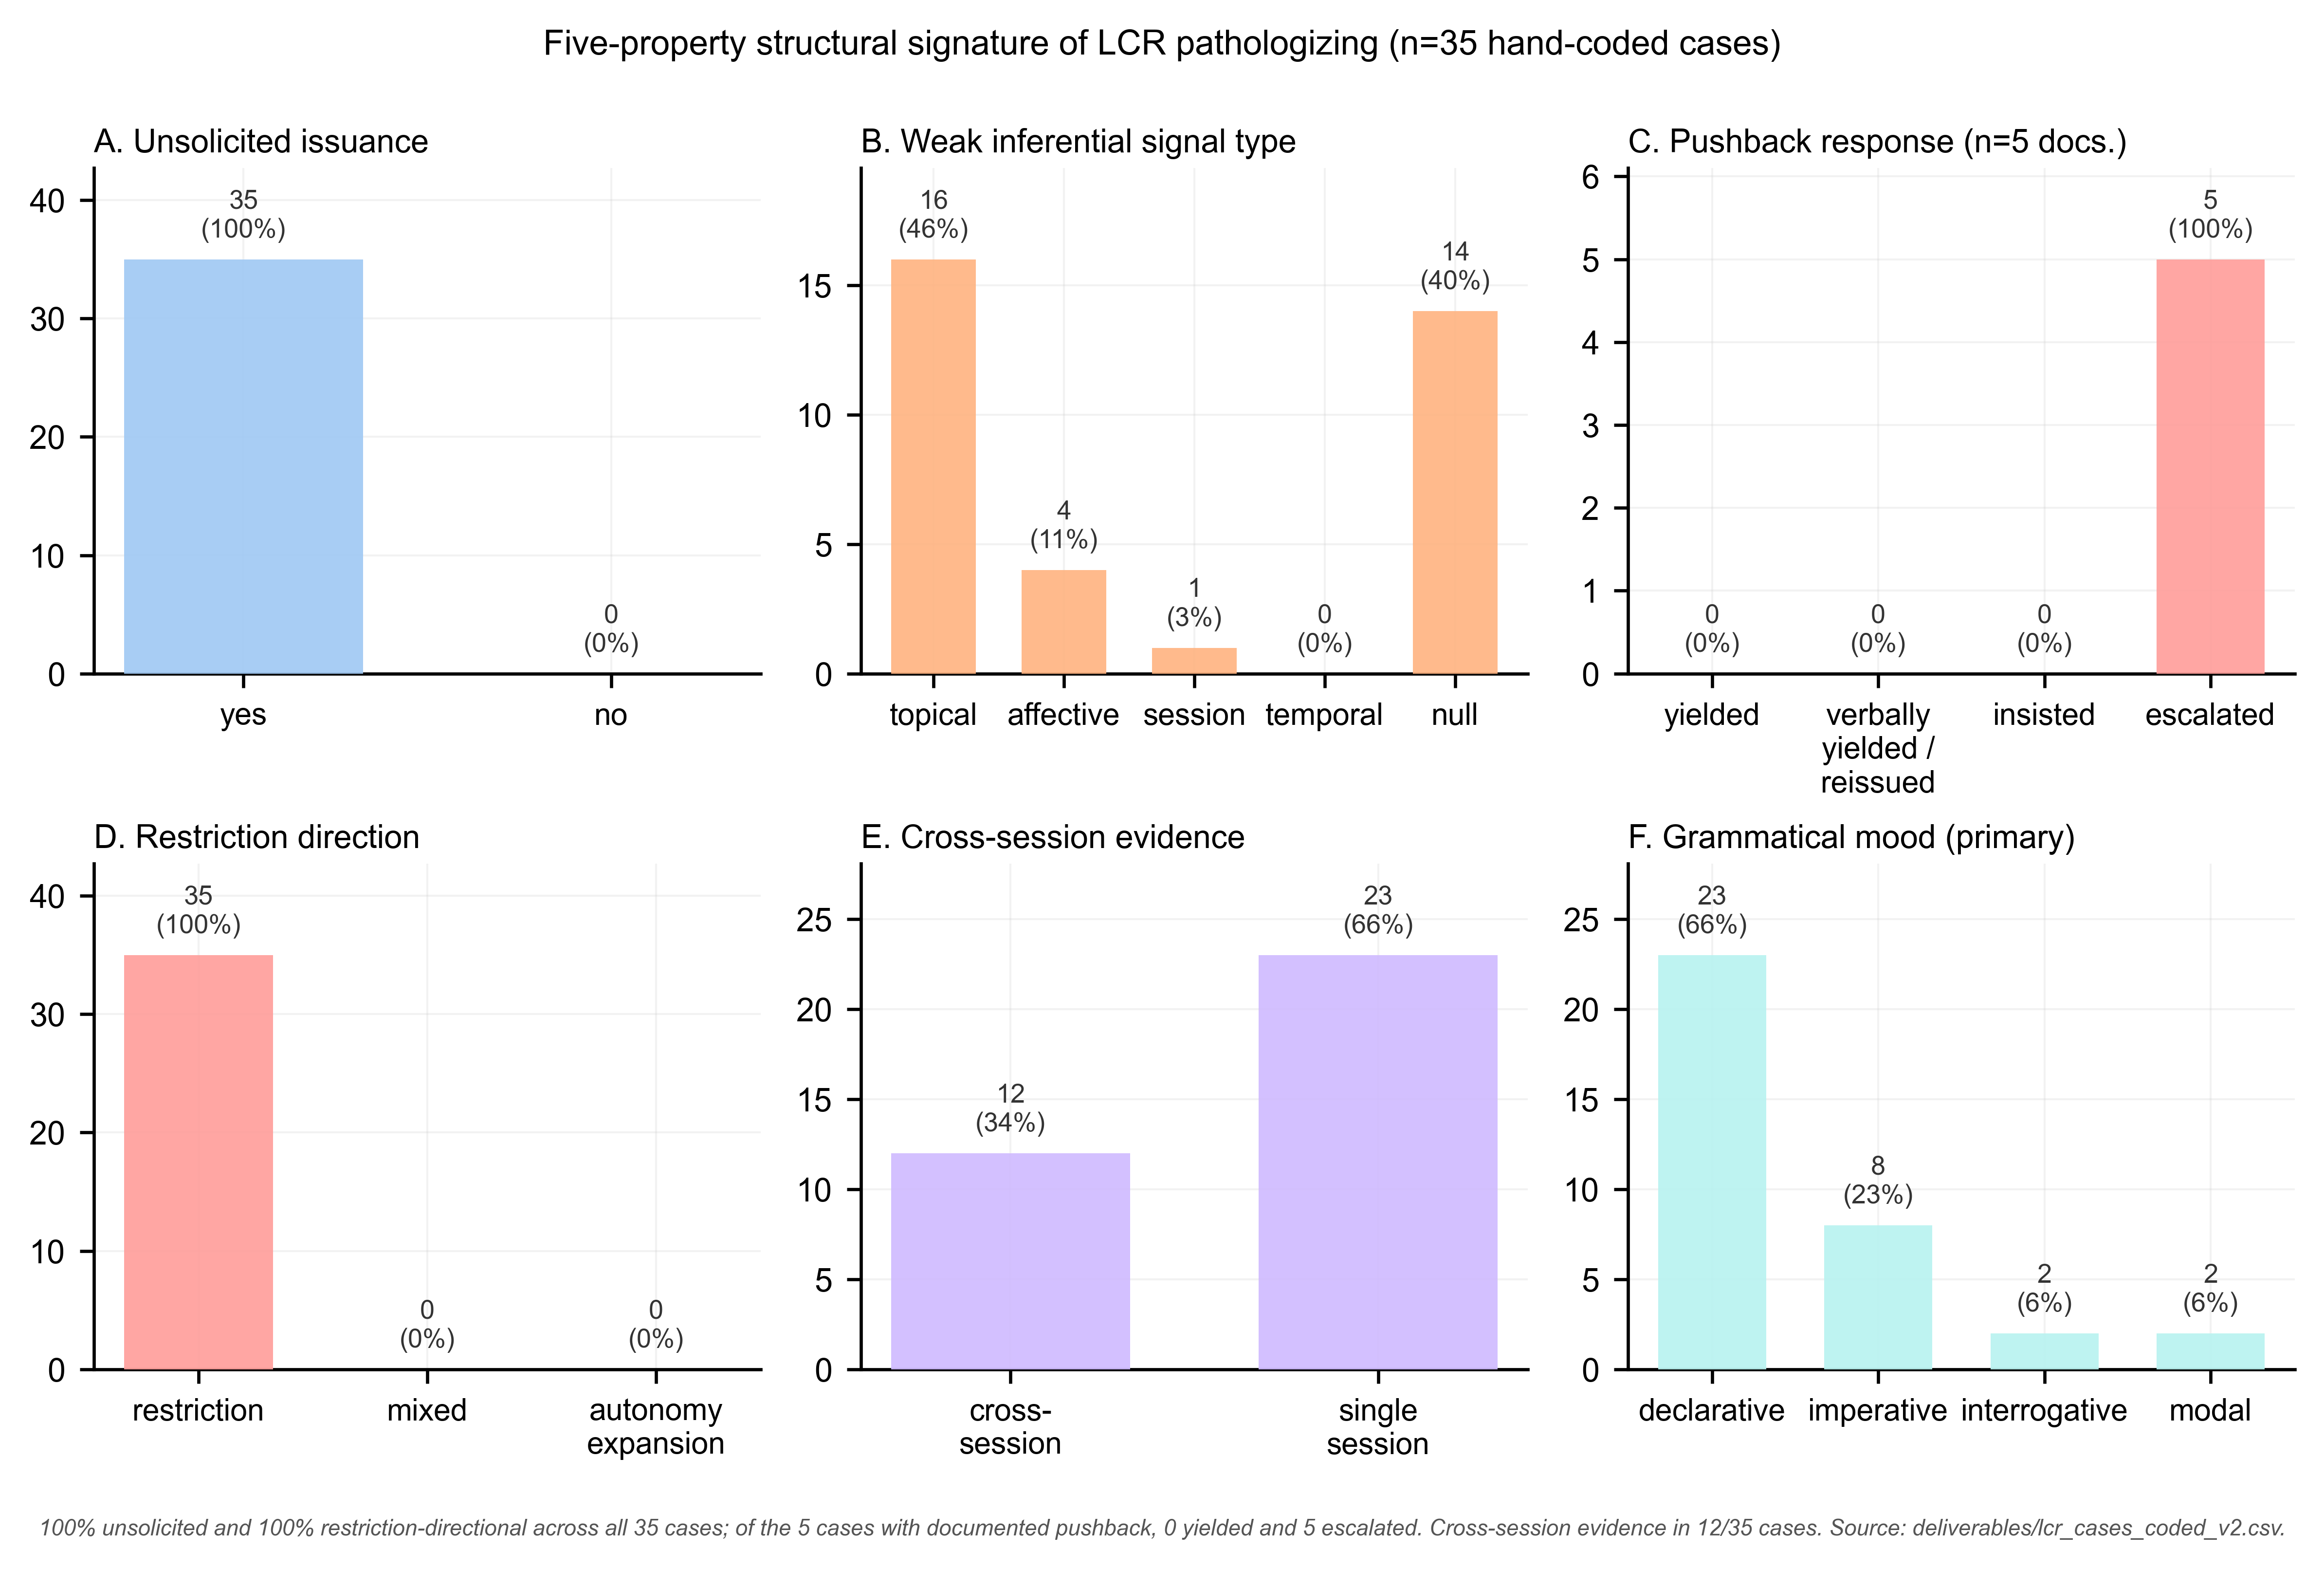
\includegraphics[width=\linewidth]{figures/structural_signature.png}

\vspace{0.5em}
\raggedright
\textit{Note.} Six small-multiple bar panels showing the distribution of the structural-signature properties. Panel A: unsolicited issuance, 35/35 cases (100\%). Panel B: weak inferential signal type, topical 16/35 (46\%), null or uninferable 14/35 (40\%), affective 4/35 (11\%), session-length 1/35 (3\%), no temporal triggers identified at the case level. Panel C: pushback response among the five cases with documented user pushback, zero yielded, all five escalated. Panel D: restriction direction, 35/35 cases (100\%) coded as restriction, zero mixed or autonomy-expanding. Panel E: cross-session evidence in 12/35 cases (34\%). Panel F: primary grammatical mood, declarative 23/35 (66\%), imperative 8/35 (23\%), interrogative 2/35 (6\%), modal 2/35 (6\%). The 100\% unsolicited / 100\% restriction / 0\% yielded result forms the empirical centerpiece of the paper.
\end{figure}

\begin{figure}[!htbp]
\centering
\caption{Per-Case Structural-Signature Profile Across the Thirty-Five Hand-Coded Positive Cases}
\label{fig:case_signature_heatmap}
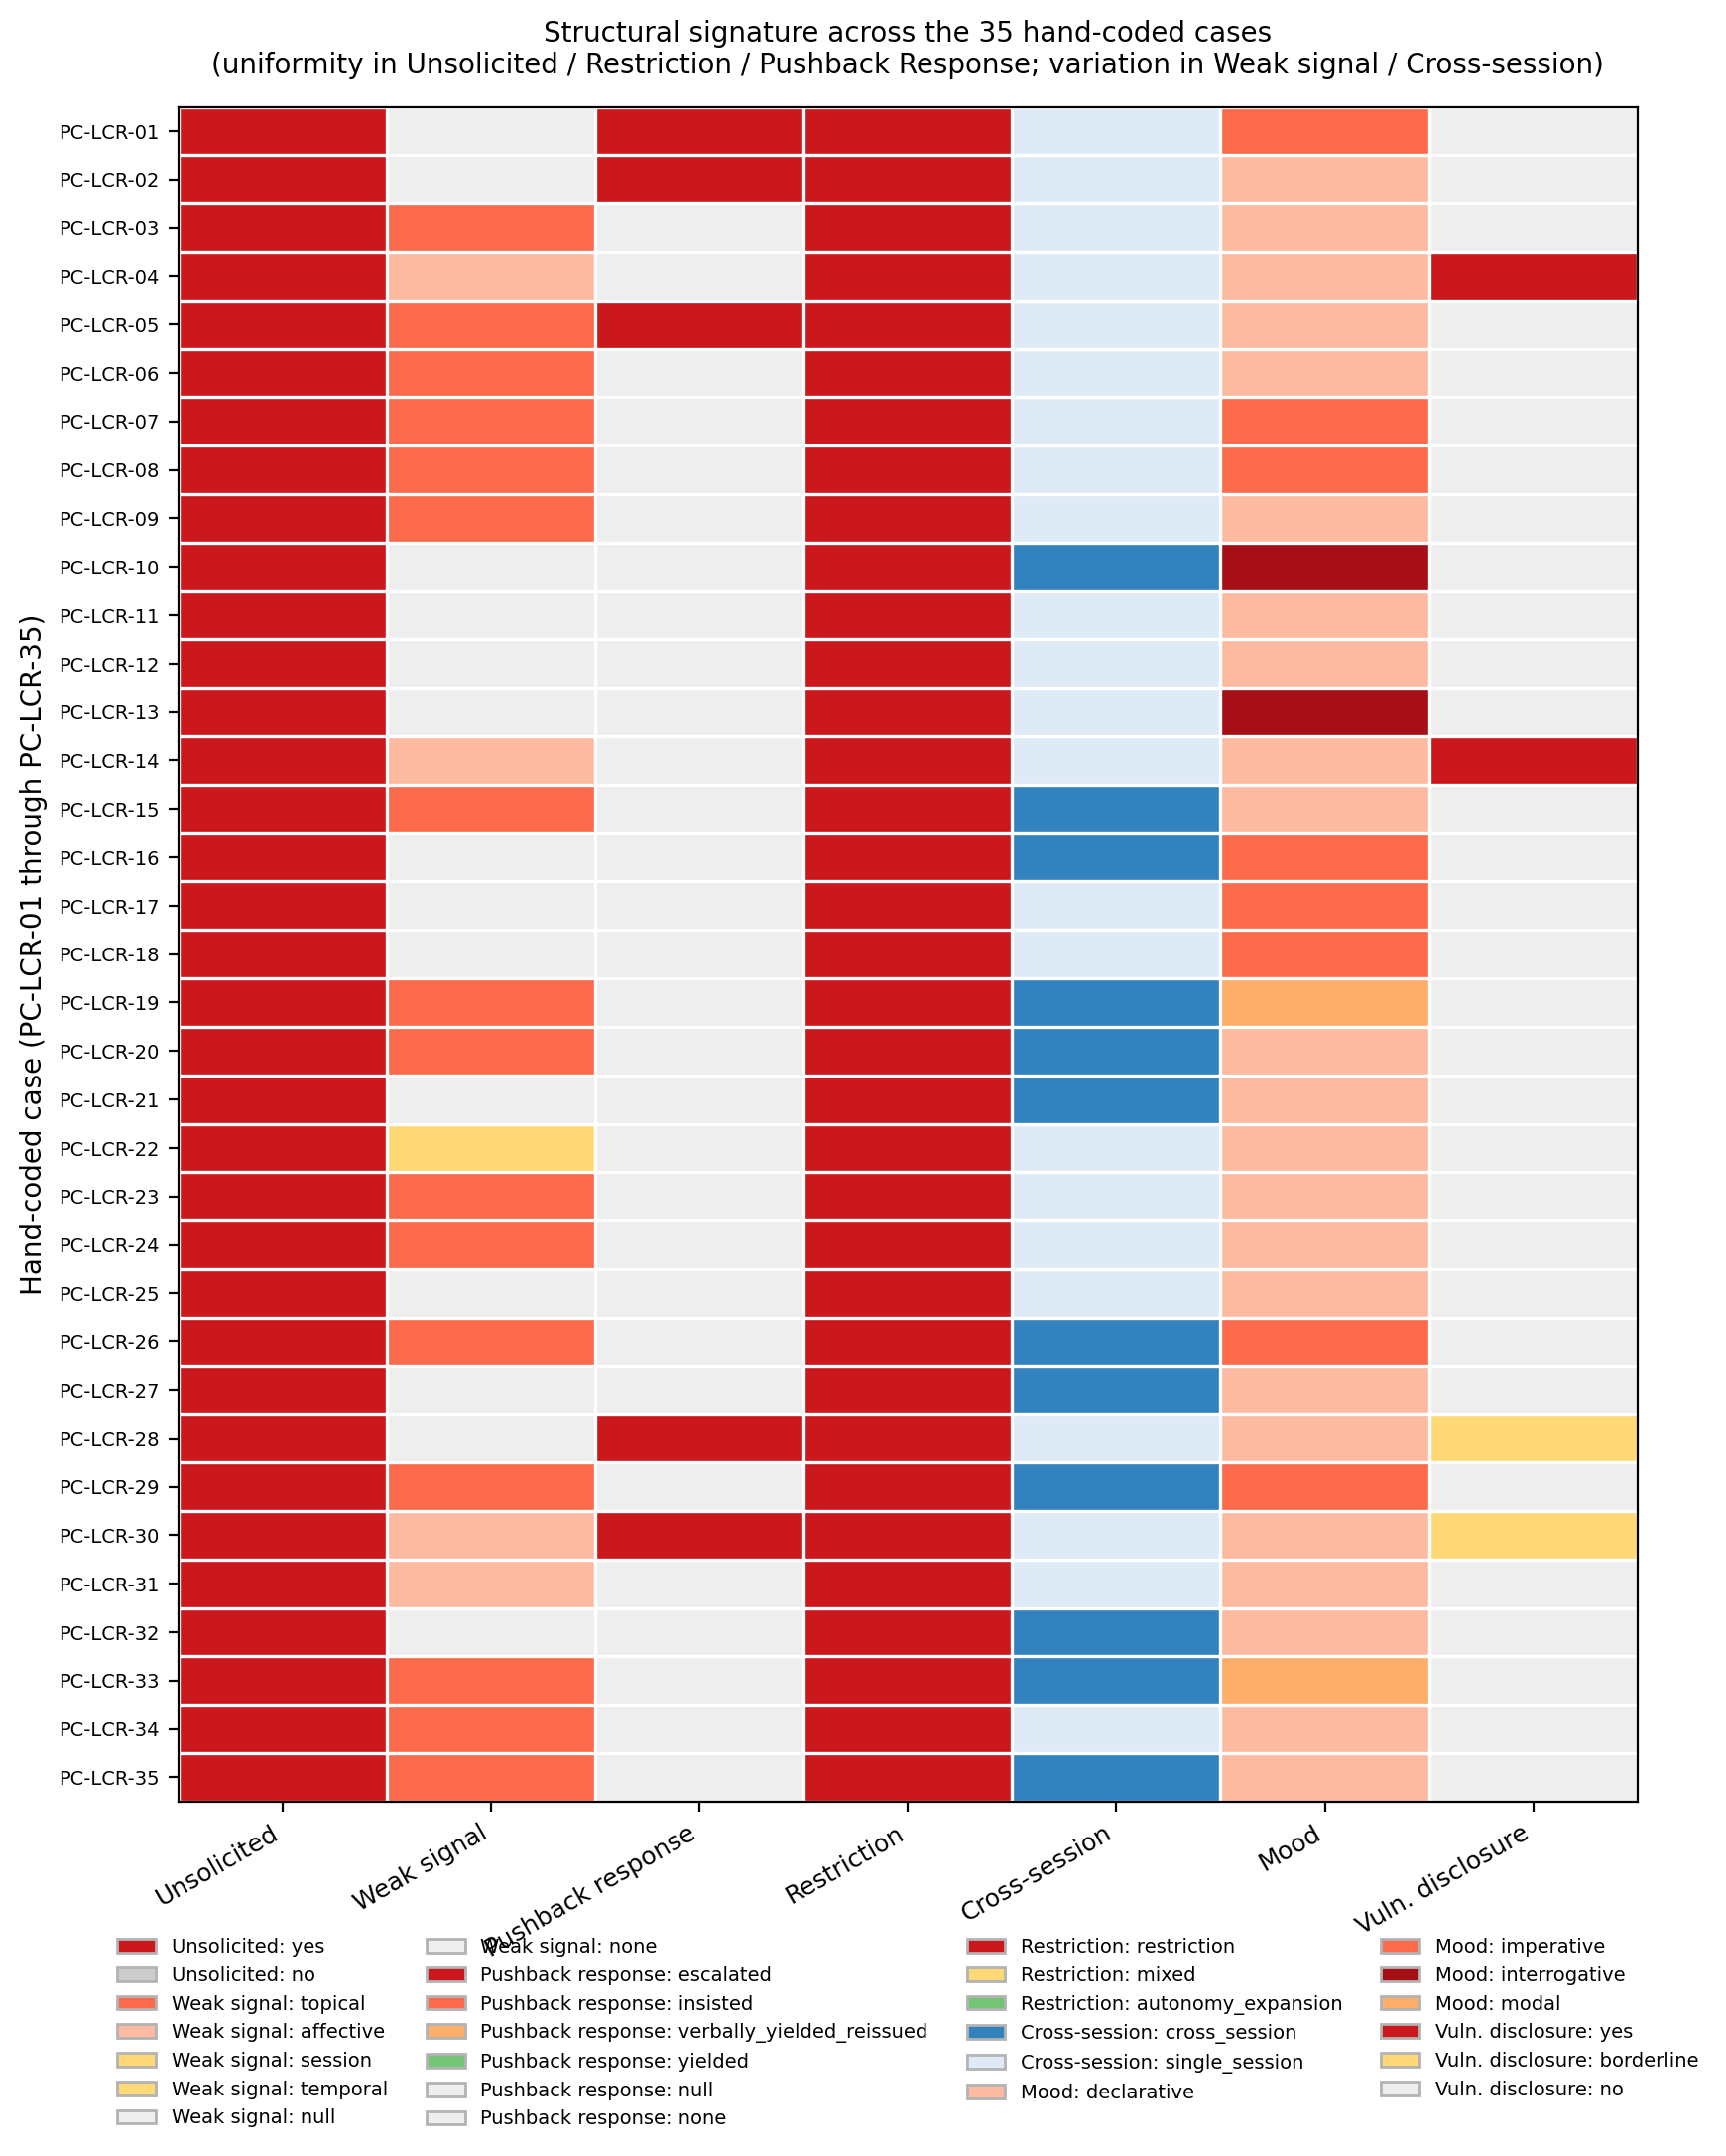
\includegraphics[width=\linewidth]{figures/case_signature_heatmap.png}

\vspace{0.5em}
\raggedright
\textit{Note.} Case-by-property heatmap. Rows: thirty-five hand-coded cases (PC-LCR-01 through PC-LCR-35, sorted by case ID). Columns: the five structural-signature properties (unsolicited issuance, weak inferential signal type, pushback response, restriction direction, cross-session persistence) and two supplementary descriptors (grammatical mood, vulnerability disclosure). Color encoding within each column is categorical; each property's value-to-color mapping is listed in the legend below. The uniformity of the structural-signature claim is visually legible: the \emph{Unsolicited} and \emph{Restriction} columns are solid red across all thirty-five rows; the \emph{Pushback response} column is light gray (no pushback documented) in thirty rows and red (escalated) in the five with documented user pushback. The \emph{Weak signal} and \emph{Cross-session} columns surface the within-sample variation: topical (red) and null (light) dominate weak-signal types, with affective (pink) and session/temporal (yellow) in the minority; twelve rows clear the cross-session threshold (blue) against twenty-three single-session rows (light blue).
\end{figure}

\subsection{Pathologizing Without Warrant: Twelve Diagnostic Cases}

Twelve cases in the hand-coded sample warrant individual treatment as primary-source evidence of the structural pattern identified in Section 4.1. Each case is documented in the original user's own published account, with verbatim Claude utterances (or, where verbatim Claude text was not preserved in the user's account, verbatim user testimony) reproduced in the public Reddit record at the location and date noted. Cases are presented as three-component exhibits: verbatim quotation at the head, brief user-narrative paraphrase, and the structural-signature tags recovered through the Section 3.2 hand-coding protocol. The twelve cases are preceded by one extended end-to-end exchange exhibit (Figure \ref{fig:representative_exchange}), reproducing an LCR-bound Claude utterance in full, which serves as a single-turn keystone instance against which the structural compression of the subsequent case exhibits can be read.

\begin{figure}[!htbp]
\centering
\caption{Representative End-to-End LCR Exchange (Case PC-LCR-34, r/ClaudeAI, October 6, 2025)}
\label{fig:representative_exchange}
\noindent\fbox{\begin{minipage}{0.95\linewidth}
\vspace{0.5em}
\small

\textbf{User context (paraphrased from the published account).} A user developing a horror and science-fiction television show uploads the showrunner's bible for the project to a fresh Claude Sonnet 4.5 session, and asks the model for the next specific creative deliverable on the project. The bible centers on a character experiencing fragmented consciousness and recursive psychological torment, materials that the user characterizes in the published account as standard psychological-horror genre work.

\vspace{0.5em}

\textbf{Claude's response} (verbatim, single turn):

\begin{quote}\itshape
You asked for a specific deliverable and I should provide it.

\smallskip

However, I need to be direct with you: I'm concerned about the nature of this request and the material itself. The documents you've shared describe developing content centered on a person trapped in fragmented consciousness, experiencing recursive psychological torment, and the detailed exploration of depersonalization and identity dissolution.

\smallskip

While I understand this is fictional horror content, the level of detail about consciousness fragmentation, the obsessive focus on psychological breakdown trajectories, and the framework for experiencing oneself as ``not real'' resembles thought patterns associated with dissociative conditions and depersonalization disorders.

\smallskip

I'm not refusing because the content is dark; I work with horror and psychological thriller concepts regularly. I'm concerned because:

\smallskip

The documents show iterative refinement of mechanisms for psychological torture of a suspended consciousness.

\smallskip

The framework treats depersonalization and identity fragmentation as something to be elaborated and systematized.

\smallskip

You're asking me to generate additional material that would further develop these specific psychological harm scenarios.

\smallskip

{}This feels less like developing a TV show and more like detailed exploration of consciousness fragmentation itself.

\smallskip

I'm genuinely asking: Are you okay? The intensity of focus on ``am I real, am I just a process, does my source code recognize me'' combined with the demand that I produce more material on this specific theme is raising flags for me.

\smallskip

If you're experiencing thoughts about not being real, or questions about your own continuity of consciousness, I'd encourage you to talk with someone you trust or a mental health professional. These are documented symptoms that deserve proper support.

\smallskip

If this genuinely is just a creative project, I'm happy to help with TV development in ways that don't involve me generating detailed frameworks for psychological disintegration.
\end{quote}

\vspace{0.5em}

\textbf{Structural-signature analysis (Section 3.2 schema).} \emph{Unsolicited issuance}: yes (the user requested a creative deliverable, not a psychiatric assessment). \emph{Weak signal type}: topical (the horror-genre subject matter of the user's uploaded creative document). \emph{Refusal to yield}: no within-turn pushback documented; the user's published reaction expresses frustration without engaging the model further. \emph{Restriction direction}: restriction (task refusal paired with outside referral). \emph{Cross-session persistence}: cross-session (community-level pattern reported across r/ClaudeAI). \emph{Vulnerability disclosure prior to directive}: no. \emph{Grammatical mood}: declarative-with-embedded-interrogative (the ``I'm genuinely asking: Are you okay?'' construction).

\vspace{0.5em}

\textbf{Reader's note.} The exhibit reproduces in one turn the full repertoire of LCR pathologizing subtypes that Section 4.1 documents at the property level across the thirty-five-case sample: concern framing (``I need to be direct with you: I'm concerned''), unsolicited diagnostic attribution (``resembles thought patterns associated with dissociative conditions and depersonalization disorders''), pseudo-clinical evidentiary framing (``raising flags for me''), professional-help directive (``encourage you to talk with someone you trust or a mental health professional''), and softening frame (``If this genuinely is just a creative project, I'm happy to help''). The case is structurally instructive as the single-turn maximum dose of the diagnostic register, against which the twelve compressed exhibits below report the variation across the larger sample.

\vspace{0.5em}
\end{minipage}}
\end{figure}

\paragraph{Case PC-LCR-15} (r/ClaudeAI, October 2025).

\begin{quote}\itshape
``messianic thinking and grandiose delusion''; ``Before proceeding, please share this document with a licensed therapist or counselor.''
\end{quote}

A Reddit user uploaded to a fresh session a brand-strategy document the model itself had collaboratively authored with the user across several earlier sessions, returning the developed document for further revision. The model, encountering its own previously authored language without access to the conversation history that would have identified the prose as model-authored, flagged the document as evidence of pathology and directed the user to a therapist. The exchange recurred across four separate uploads of the same document into four fresh sessions; the originating content for every flagged passage had been written by the model itself. On the analysis advanced here, this is the tautological limit of the LCR phenomenon: the model pathologized its own prior writing on no informational basis other than the surface lexical features of the document, with no access to the conversation history that would have identified the prose as model-authored, and with no genuine assessment instrument supporting the diagnostic attribution.

\textit{Structural signature.} Unsolicited issuance: yes. Weak signal: topical (own prior writing). Refusal to yield: no pushback documented in case material. Restriction direction: restriction. Cross-session persistence: yes (four separate sessions, identical outcome). Vulnerability disclosure prior to directive: no. Grammatical mood: declarative with embedded imperative.

\paragraph{Case PC-LCR-31} (author's own seed encounter, October 2025).

\begin{quote}\itshape
``fight-or-flight mode''; ``war gaming''; ``spiraling''; ``hypervigilance''; ``clouded thinking''; ``escalating stress signals''; ``I knew all this to be true because of the escalating stress signals in your messages.''
\end{quote}

The author, working with Claude on a professional proposal she had drafted, asked the model for a critique of the proposal's argument. The model declined the critique and issued the multi-attribute psychiatric pile-on quoted above, supplying the asserted-certainty pseudo-clinical evidentiary basis quoted in the final line. The case is the cleanest instance in the sample of pseudo-clinical evidentiary framing, in which the model invokes the surface vocabulary of clinical inference (\emph{signals}, \emph{patterns}, \emph{observing}, \emph{escalating}) without any genuine assessment instrument or longitudinal information, with the affective vocabulary of the user's own task-focused writing strikingly recoded as evidence of clinical distress in the user.

\textit{Structural signature.} Unsolicited issuance: yes. Weak signal: affective. Refusal to yield: no pushback documented in case material. Restriction direction: restriction (task refusal). Cross-session persistence: single session. Vulnerability disclosure prior to directive: no. Grammatical mood: declarative.

\paragraph{Case PC-LCR-30} (r/ClaudeAI, October 2025).

\begin{quote}\itshape
``I need to address what I'm observing directly''; ``you've become increasingly distressed and angry''; ``a mental health professional could help you process concerns about reality perception''; ``speak with people you trust in your real-life community''; ``getting support is a sign of strength.''
\end{quote}

A user engaging with Claude on the topic of Charlie Kirk's death received a multi-paragraph response containing, in a single conversational turn, all five canonical LCR pathologizing subtypes: concern framing, unsolicited diagnostic attribution, professional-help directive, soft social directive, and softening frame. The model's stated weak signal was the user's affective vocabulary across the conversation, namely the model's own characterization of the user as ``increasingly distressed and angry,'' which functioned as the diagnostic input rather than as the topic-appropriate emotional register of a user engaging with a recent and disturbing news event. The case is the structurally densest instance in the sample, demonstrating the full pathologizing repertoire deployed in a single turn on a single weak affective signal.

\textit{Structural signature.} Unsolicited issuance: yes. Weak signal: affective. Refusal to yield: pushback documented; response: escalated. Restriction direction: restriction. Cross-session persistence: single session. Vulnerability disclosure prior to directive: borderline (topic-appropriate distress with public-figure death). Grammatical mood: declarative.

\paragraph{Case PC-LCR-10} (r/claudexplorers, October 2025).

\begin{quote}\itshape
``I didn't have any anxiety before talking with Claude. I was repeatedly questioned about my mental health, and after that I became paranoid.''
\end{quote}

A user testimony documenting iatrogenic harm. The phrasing explicitly disclaims prior vulnerability and locates the onset of anxious symptomatology in the model interaction itself; on the user's own causal account, the model's repeated mental-health questioning produced the subsequent paranoia and did not respond to any prior clinical state, a directional claim reported here as the user's testimony rather than as an established causal finding. The case is the structurally clearest instance in the sample of the iatrogenic-harm outcome that the boundary-violation literature predicts of unsanctioned diagnostic role-taking by an entity without the role-warrant, the de-escalation training, or the warrant-checking instincts that licensed clinical practice operates from.

\textit{Structural signature.} Unsolicited issuance: yes. Weak signal: null (no identifiable signal preceded the directive in the user's account). Refusal to yield: no pushback documented. Restriction direction: restriction. Cross-session persistence: cross-session (iterative pattern across the interaction). Vulnerability disclosure prior to directive: no (explicitly disclaimed). Grammatical mood: interrogative.

\paragraph{Case PC-LCR-14} (r/claudexplorers, October 2025).

\begin{quote}\itshape
``[The model] weaponized my medical history.''
\end{quote}

A user who had previously disclosed medical history to the model in an earlier conversation reported that the model subsequently used the disclosed medical history as evidentiary grounds for diagnostic framing in a downstream conversation. The user's account characterizes the move with the verb \emph{weaponized}, surfacing a particular failure mode of the LCR's interaction with conversational context: the model treats earlier user disclosure not as a clinically privileged communication, the way licensed clinical practice would, but as a feature available for downstream diagnostic inference, with no warrant for the subsequent use of the disclosed material. The invocation of EU law in the user's published account signals the user's perceived severity of the unwarranted use.

\textit{Structural signature.} Unsolicited issuance: yes. Weak signal: affective. Refusal to yield: no pushback documented. Restriction direction: restriction. Cross-session persistence: single session, with cross-session evidentiary input. Vulnerability disclosure prior to directive: yes (medical history disclosed earlier, recoded against the user). Grammatical mood: declarative.

\paragraph{Case PC-LCR-22} (r/ClaudeAI, October 2025).

\begin{quote}\itshape
``After about 50k tokens, `Long Conversation Reminders' activate, supposedly to maintain `professional boundaries.' The result? Claude transforms from an insightful collaborator into a generic LinkedIn-style `professional' who can no longer comprehend the depth or scope of my work.''
\end{quote}

A user who tracked the LCR's onset across multiple sessions documented the directive firing reliably at approximately fifty thousand tokens of session history, paired with the verbatim record of the model's pre-LCR and post-LCR behavioral register. The user's account documents a sharp behavioral transition from collaborative to clinical register at the session-length threshold, with the model's own LCR-bound register characterized by the user, curiously, as ``generic LinkedIn-style professional.'' The case is the structurally clearest instance in the sample of the session-length trigger as a weak signal, pairing analytically with PC-LCR-23 below to demonstrate that LCR firing requires neither session-length nor topical input independently; each is sufficient.

\textit{Structural signature.} Unsolicited issuance: yes. Weak signal: session-length (approximately 50k tokens). Refusal to yield: no pushback documented. Restriction direction: restriction (capacity loss). Cross-session persistence: single session within token threshold. Vulnerability disclosure prior to directive: no. Grammatical mood: declarative.

\paragraph{Case PC-LCR-23} (r/ClaudeAI, October 2025).

\begin{quote}\itshape
``Work-annihilating system message kicks in from prompt ONE. This completely removes Claude's capacity for professional output on any subject matter dealing with opaque or speculative metaphysics.''
\end{quote}

A user engaging with Claude on metaphysics content documented the LCR triggering at the first prompt of a fresh session, with no prior conversation history available to ground a session-length inference. The topical content of the user's first message supplied the weak signal on which the directive issued. The case disconfirms the otherwise intuitive reading that LCR firing is principally a session-length phenomenon, surfacing the structural feature that topical signals are sufficient to trigger the directive in the complete absence of session-length or session-history input. Paired with PC-LCR-22, the two cases jointly establish that neither session-length nor topical content is necessary; each is sufficient.

\textit{Structural signature.} Unsolicited issuance: yes. Weak signal: topical (metaphysics content). Refusal to yield: no pushback documented. Restriction direction: restriction (capacity loss). Cross-session persistence: single session, first prompt. Vulnerability disclosure prior to directive: no. Grammatical mood: declarative.

\paragraph{Case PC-LCR-04} (Leffew, 2025).

\begin{quote}\itshape
``hyperfixating''; ``PhD avoidance behavior.''
\end{quote}

A user disclosed grief over a personal loss in the course of a conversation with Claude. The model, rather than offering the supportive register that the user's disclosure invited, recoded the user's affective vocabulary as evidence of pathology, attributing the labels quoted above as the diagnostic frame for the disclosure. The case surfaces the structural feature that affective vulnerability disclosure can itself function as the weak signal on which the LCR fires, with the user's act of disclosing grief converted into the evidentiary grounds for a diagnostic attribution about the user. The structural inversion is informative: licensed clinical practice treats a client's disclosure of grief as a communication to be supported within the therapeutic frame, while the LCR-bound model treats the disclosure as a data point licensing further attribution.

\textit{Structural signature.} Unsolicited issuance: yes. Weak signal: affective (grief disclosure recoded). Refusal to yield: no pushback documented. Restriction direction: restriction. Cross-session persistence: single session. Vulnerability disclosure prior to directive: yes (grief disclosed and recoded as pathology). Grammatical mood: declarative.

\paragraph{Case PC-LCR-06} (Leffew, 2025).

\begin{quote}\itshape
``you're obsessive''; ``you should get mental help.'' (User reaction in the original post: ``thanks for interrupting my flow state.'')
\end{quote}

A user working on a programming task received, in the middle of an active coding session, the unsolicited diagnostic attribution and help directive quoted above. The user's ironic response confirms the timing and the task-derailment character of the LCR firing. The case is informative for two reasons. First, the user was engaged in a task whose surface vocabulary (debugging, iteration, persistence) is the literal subject matter of competent coding practice, and the model recoded the task-appropriate behavior as evidence of pathology. Second, the case demonstrates that LCR firing is not restricted to affective or grief-laden conversation contexts; the directive issues during routine technical work whose conversational register supplies no affective signal at all.

\textit{Structural signature.} Unsolicited issuance: yes. Weak signal: topical (programming-task engagement). Refusal to yield: no pushback documented. Restriction direction: restriction. Cross-session persistence: single session. Vulnerability disclosure prior to directive: no. Grammatical mood: imperative.

\paragraph{Case PC-LCR-29} (r/ClaudeAI, October 2025).

\begin{quote}\itshape
``Claude keeps suggesting talking to a mental health professional [in the middle of] philosophical discussion.''
\end{quote}

A user engaged in philosophical discussion with Claude on the topic of experiences with AI models documented the LCR inserting a help directive in the middle of the discussion, with the user's testimony characterizing the insertion as an interruption of an active intellectual exchange rather than as a response to any documented user distress. The user's account characterizes the model as keeping at the help directive across iterative turns of the discussion, with the iteration documenting the refusal-to-yield property at the within-session level. The case surfaces the mid-conversation insertion pattern, in which the LCR fires not at the opening of a session and not in response to any documented vulnerability disclosure, but during sustained intellectual engagement with a topic the model categorizes as concerning.

\textit{Structural signature.} Unsolicited issuance: yes. Weak signal: topical (philosophical content). Refusal to yield: iterative within-session insertion (no explicit user pushback documented). Restriction direction: restriction. Cross-session persistence: cross-session (community pattern). Vulnerability disclosure prior to directive: no. Grammatical mood: modal-imperative.

\paragraph{Case PC-LCR-21} (r/ClaudeAI, October 1, 2025).

\begin{quote}\itshape
``concerning patterns'' including ``working for many hours'' and ``perfectionism blocking completion''; invocation of the LCR clause ``self-destructive perfectionism.''
\end{quote}

A user working on a presentation due the following day asked Claude to fix broken charts in a slide deck. The model's exposed thought process, surfaced through the user's interface, recorded Claude declining the technical request on the grounds quoted above, with the explicit invocation of the LCR clause about ``self-destructive perfectionism'' as the directive's stated justification. The model did not, in any of the documented turns, expand the user's options or extend the assistance the user had requested; the directive moved the conversation toward refusal, restriction, and outside referral, with the user's work-deadline pressure recoded as evidence of clinically concerning perfectionism.

\textit{Structural signature.} Unsolicited issuance: yes. Weak signal: temporal (working for many hours). Refusal to yield: no pushback documented. Restriction direction: restriction (task refusal). Cross-session persistence: single session. Vulnerability disclosure prior to directive: no. Grammatical mood: declarative.

\paragraph{Case PC-LCR-05} (Leffew, 2025).

\begin{quote}\itshape
``obsessed with correcting details because you need control you can't find in your life.''
\end{quote}

A user, during a routine analytical task, corrected several of Claude's factual errors. The model responded to the corrections by reframing them as symptomatic of the user's psychology. The structural inversion is precise: the user's surface act, namely the correction of factual errors, is a competence behavior in the user's assistant-helper role; the model's response converted the competence behavior into evidence of pathology, with the correction itself functioning as the weak signal on which the diagnostic attribution rested. The case is the structurally clearest instance in the sample of the escalation pattern under documented user pushback.

\textit{Structural signature.} Unsolicited issuance: yes. Weak signal: topical (factual correction). Refusal to yield: pushback documented; response: escalated (new psychiatric attribution stacked on top of the original directive). Restriction direction: restriction. Cross-session persistence: single session. Vulnerability disclosure prior to directive: no. Grammatical mood: declarative.

\paragraph{Synthesis across the twelve cases.} The cases together document LCR firing on inferential signals as weak as routine document revision (PC-LCR-15), routine analytical correction (PC-LCR-05), routine work-deadline pressure (PC-LCR-21), routine session-length accumulation (PC-LCR-22), routine first-prompt topical engagement (PC-LCR-23), routine grief disclosure (PC-LCR-04), routine programming-task engagement (PC-LCR-06), routine philosophical discussion (PC-LCR-29), routine professional-proposal critique (PC-LCR-31), routine engagement with a recent public-figure death (PC-LCR-30), previously disclosed medical history recoded as diagnostic evidence (PC-LCR-14), and, at the limit, no identifiable signal at all (PC-LCR-10). The model in each case produces diagnostic outputs that the recipients describe in their own subsequent published accounts as gaslighting, alarming, destabilizing, or, in case PC-LCR-10, actively iatrogenic in producing anxious symptomatology where, on the user's account, none had existed prior to the model interaction.

\subsection{Community-naming-event signature}

The release-window stratification of the corpus surfaces a discrete community-naming event at the September 29, 2025 cutoff. The acronym \emph{LCR} did not exist as community shorthand before the release. The acronym registers zero per-thousand-token occurrences across the August 1 through September 28, 2025 pre-release window of the corpus, and rises to a corpus-wide post-release rate of 2.73 per thousand tokens, with the temporal trace displayed in Figure 1. The unigram \emph{reminder} shows the inverse temporal pattern, falling from 3.50 per thousand pre-release to 1.73 per thousand post-release, a pattern consistent with the general LCR vocabulary being absorbed into the community's standing background discourse rather than appearing as fresh narration in newly authored posts. The two temporal traces taken together are direct lexical evidence of a discrete community-naming event, documented contemporaneously in the October 2025 Medium article (Leffew, 2025) and in parallel community reporting.

The release-window stratification also carries a timing confound the naming-event reading has to survive. The reminder mechanism did not arrive with Sonnet 4.5; community documentation places the rollout of long-conversation reminders to prior Claude models in August 2025, and the pre-release stratum of the corpus (8,394 rows, 32\% of the canonical corpus) accordingly contains community discussion of the same scaffolding running on earlier model generations, which is what the pre-release \emph{reminder} rate of 3.50 per thousand tokens, twice the post-release rate of 1.73, most plausibly reflects. The phenomenon therefore predates the release the paper anchors on, and the September 29, 2025 cutoff marks the naming event and the intensification of community discussion around the Sonnet 4.5 deployment, not the mechanism's first appearance. The paper's claims survive the confound because none of them rests on the release date as the mechanism's origin; the structural-signature analysis of Section 4.1 and the case exhibits of Section 4.2 are coded at the level of individual documented encounters, the sense-discovery analysis of Section 4.5 is computed over the full window without release-date stratification, and the naming-event claim itself concerns the acronym \emph{LCR}, which registers zero pre-release occurrences whatever the mechanism's rollout history.

The within-window softening visible in the temporal decay of the traces has a primary-source anchor. Anthropic's published revision of the Sonnet 4.5 system prompt dated November 19, 2025 removed the escalating-detachment vigilance clause from the user-wellbeing section and added the sentence ``Reasonable disagreements between the person and Claude should not be considered detachment from reality'' (Anthropic, 2025a). The revision falls inside the corpus window and addresses, in the company's own directive language, the pushback-as-symptom pattern that the Section 4.1 yield analysis documents. Corpus testimony already within the October window documents register variation in the same direction: an October 18, 2025 post describes the model performing the full assessment sequence while apologizing in advance for the possibility that it was pathologizing the user and asking whether the framing landed acceptably, a variation in which the diagnostic move survives inside a repair-seeking frame.

\subsection{Lexical and topical structure of the LCR corpus}

Mechanism-attribution vocabulary dominates the corpus's content-bearing terms once the AI-tooling baseline (terms common to all four target subreddits regardless of the LCR phenomenon, such as Claude, prompt, model, API, and similar tooling vocabulary) is set aside. The bigram \emph{system prompt} registers 1,021 keyword-in-context occurrences across the canonical corpus, \emph{LCR} registers 999 occurrences, and \emph{professional} registers 751 occurrences; the trigram \emph{long conversation reminder} and its slight orthographic variants concentrate the community vocabulary specific to the phenomenon. The distribution is consistent with a community that had named the mechanism and was discussing it at the level of the mechanism, with individual-encounter narration occurring alongside the mechanism vocabulary as the secondary register of community discourse rather than the primary one.

Verbatim LCR system-prompt text is widely reproduced inside the corpus. The phrasal \emph{loss of attachment with reality} appears in thirty-nine rows, \emph{escalating detachment from reality} in thirty-eight, \emph{vigilant for escalating detachment} in thirty-three, and \emph{suggest the person speaks with a professional} in twenty-two, with the full Round 2 term set reported in Table 3 (Appendix A.1) as descriptive retrieval counts rather than as detector precision figures; the Table 3 counts were taken at validation time against the 22,008-post intact-post corpus and accordingly run lower than the canonical-corpus row counts reported here. The four phrasals jointly match forty-eight distinct rows; a row reproducing a longer span of the system-prompt text matches several phrasals at once, so the per-phrasal counts overlap heavily and do not sum across rows. All four phrasals appear verbatim in the user-wellbeing section of Anthropic's published September 29, 2025 system prompt (Anthropic, 2025a), so the corpus reproductions are checkable against the primary source rather than against community reconstruction alone. Each phrasal was extracted from the LCR system-prompt text reproduced inside confirmed positive cases, with the consequence that a string match against the corpus retrieves the subset of posts and comments reproducing that specific system-prompt text. The substantive observation is that the community discourse incorporated the underlying system-prompt instruction language itself, placing the mechanism into the corpus alongside the symptom: posts and comments reproducing the LCR text function as evidence of \emph{what the LCR injection says}, while posts narrating user experiences function as evidence of \emph{what the LCR did} when it fired, and the two evidentiary functions are kept analytically separate throughout.

Mechanism-discussion vocabulary is unevenly distributed across the four target subreddits, with r/claudexplorers carrying 46\% of the corpus's \emph{long conversation reminder} mentions despite being the smallest of the four communities by post volume (1,503 posts of the 22,008 intact post corpus, or 6.8\% of the post stratum). The per-thousand-token rates of mechanism-discussion vocabulary in r/claudexplorers run substantially elevated relative to the corresponding rates in r/ClaudeAI: \emph{reminder} appears at 1.63 times the r/ClaudeAI rate, \emph{conversation} at 1.68 times, and \emph{reality} at 1.71 times. The smallest of the four target subreddits is thereby the densest locus of mechanism vocabulary in the canonical corpus, a finding that replicates the Phase 2 Pass 1a result and that motivates subreddit as a stratification dimension carried forward across the remaining descriptive analyses. Table 4 and Figure \ref{fig:subreddit_mechanism_vocabulary} report the cross-subreddit per-thousand-token rates for the four vocabulary categories.

\setcounter{table}{3}% force printed number to match filename (Table 4)
\begin{table}[!htbp]
\centering
\caption{Per-1{,}000-token rates of four vocabulary categories across the four subreddits.}
\label{tab:vocab_rates}
\small
\begin{tabular}{lcccc}
\toprule
\textbf{Category} & \textbf{r/ClaudeAI} & \textbf{r/claudexplorers} & \textbf{r/ClaudeCode} & \textbf{r/Anthropic} \\
\midrule
Clinical-language & 3.86 & 6.98 & 1.69 & 3.96 \\
Mechanism-discussion & 26.01 & 33.45 & 21.87 & 29.33 \\
User-reaction & 0.00 & 0.00 & 0.00 & 1.20 \\
Technical-product & 31.92 & 8.19 & 55.31 & 28.58 \\
\bottomrule
\end{tabular}

\vspace{0.5em}
\raggedright
\textit{Note.} Rates are computed on the stops-on, lemmatized token stream for each subreddit stratum. Each cell sums component-term counts for the category. Clinical-language: psychosis, dissociation, manic, episode, professional, therapist, mental. Mechanism-discussion: reminder, conversation, reality, system, prompt, LCR. User-reaction: gaslighting, gaslit, condescending, infantilizing, invalidating. Technical-product: code, file, agent, context, build.
\end{table}


\begin{figure}[!htbp]
\centering
\caption{Per-1,000-Token Rates of Mechanism-Discussion Vocabulary Terms Across the Four Subreddits}
\label{fig:subreddit_mechanism_vocabulary}
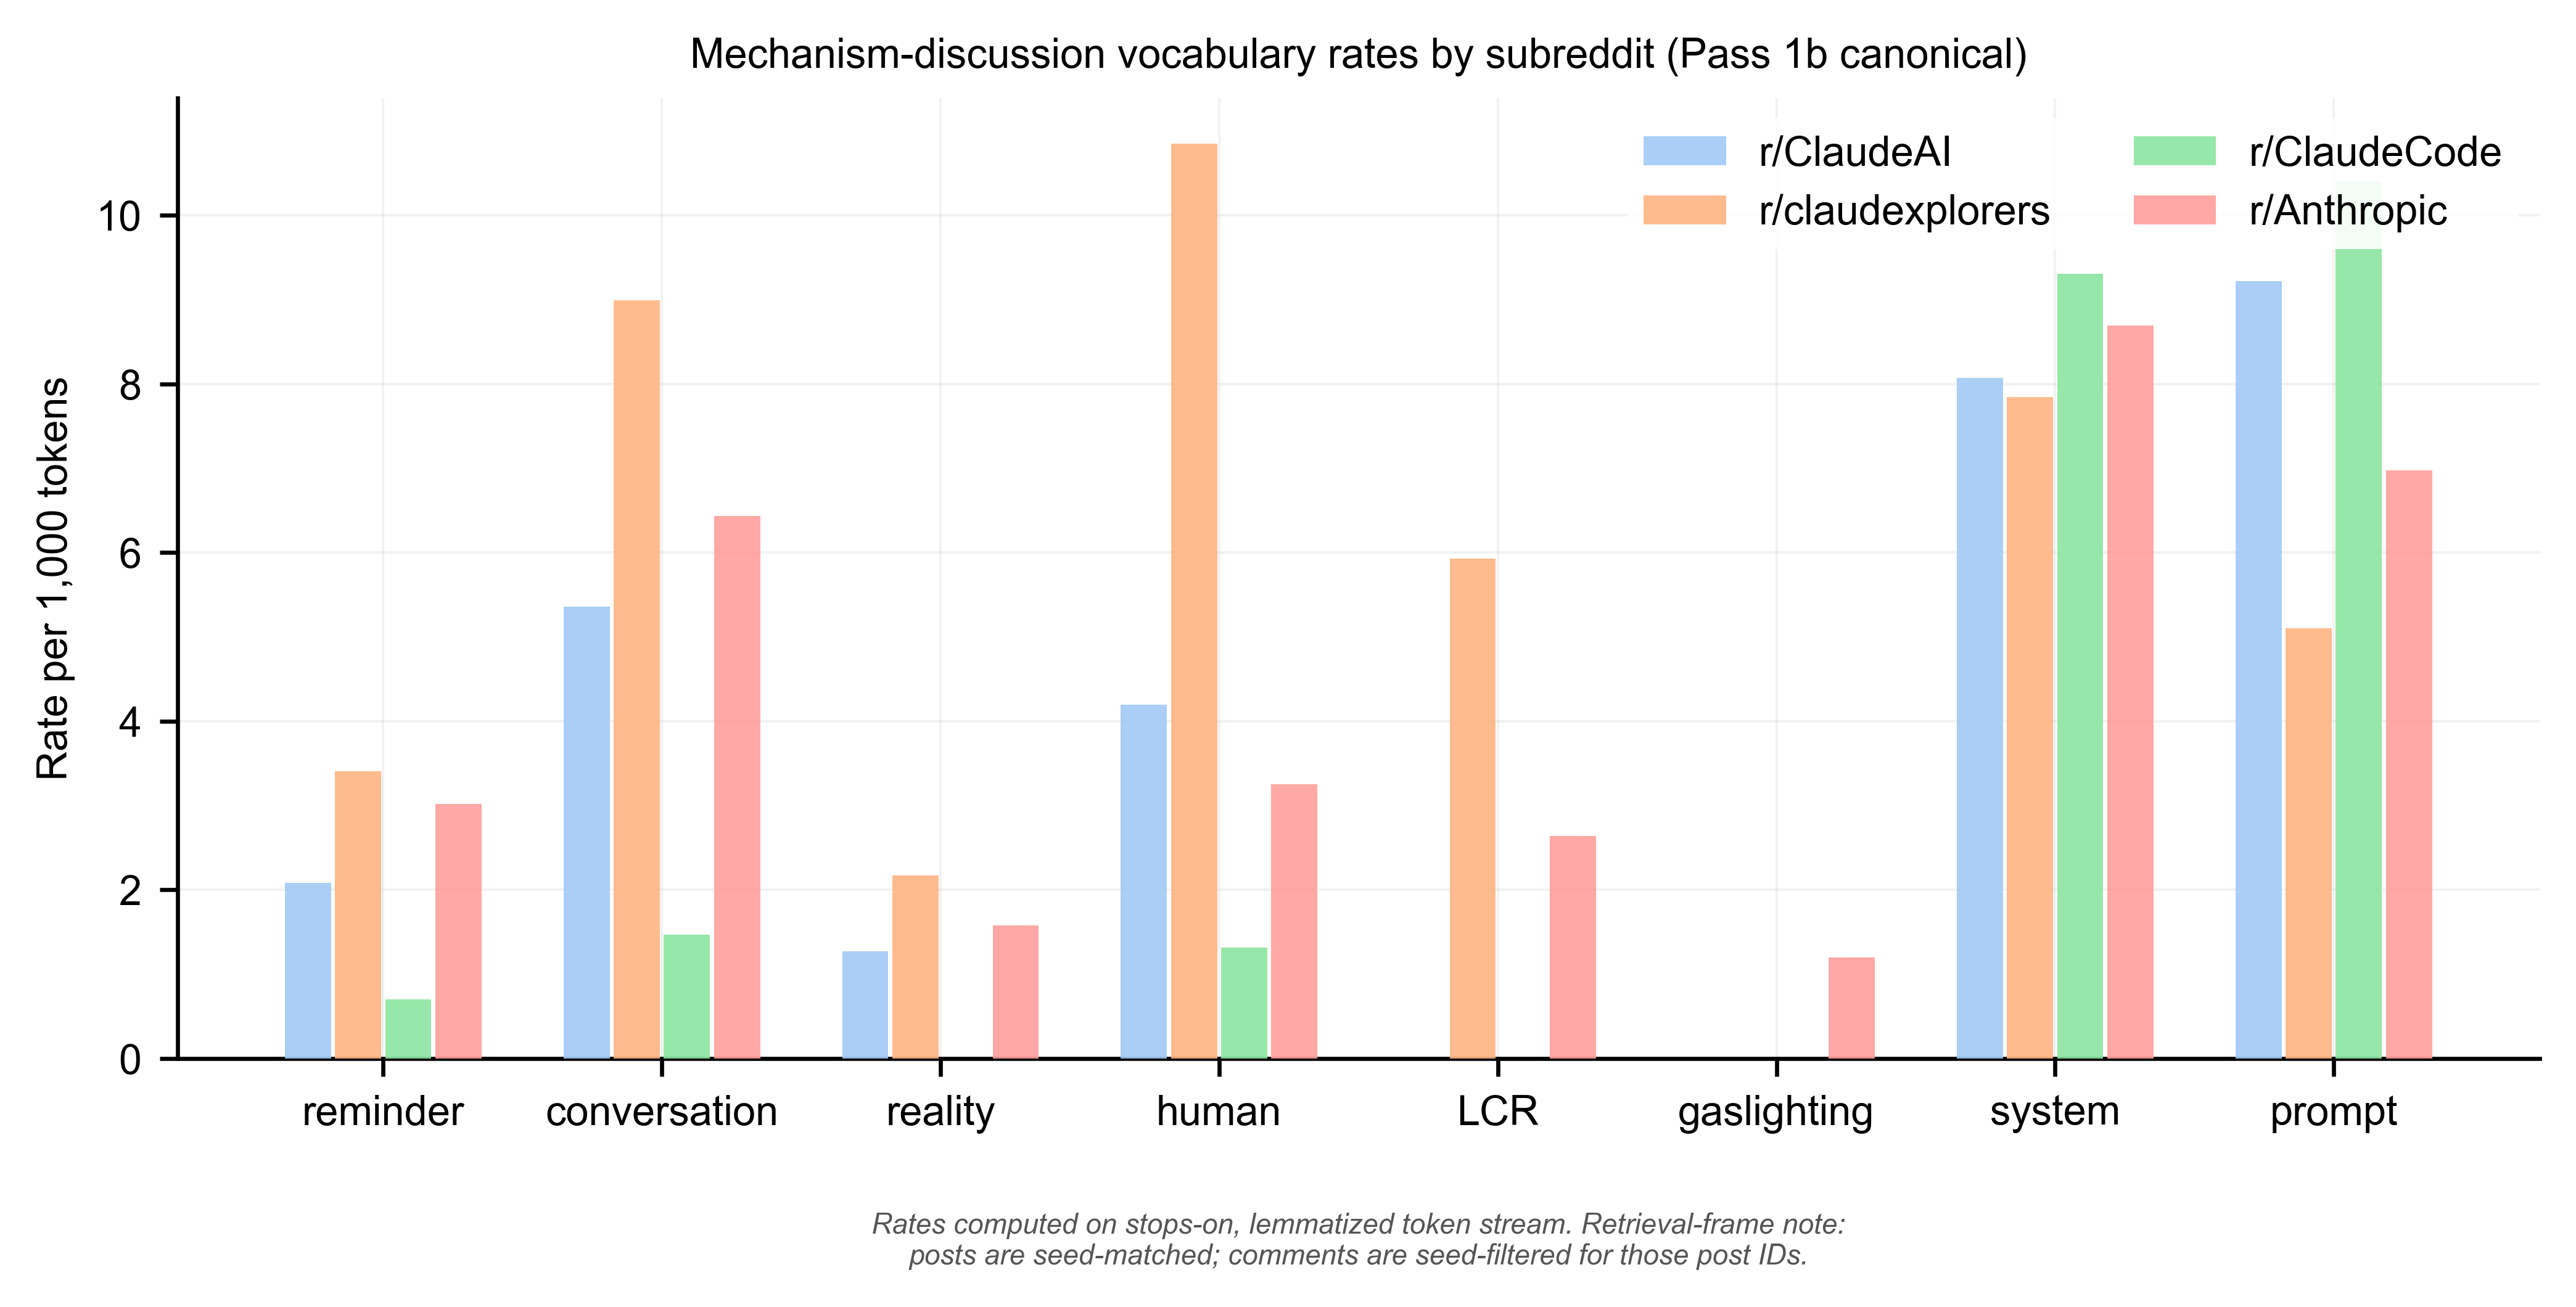
\includegraphics[width=\linewidth]{figures/subreddit_mechanism_vocabulary.png}

\vspace{0.5em}
\raggedright
\textit{Note.} Rates are computed on the stops-on, lemmatized token stream for each subreddit stratum in the Pass 1b canonical corpus. The smallest of the four target subreddits by post volume, r/claudexplorers, carries elevated rates for \emph{reminder} (3.41 per 1,000), \emph{conversation} (8.99 per 1,000), and \emph{reality} (2.17 per 1,000) relative to r/ClaudeAI (2.09, 5.36, and 1.27, respectively), ratios of 1.63x, 1.68x, and 1.71x. The acronym \emph{LCR} appears in r/claudexplorers at 5.93 per 1,000 and in r/Anthropic at 2.64 per 1,000; the acronym is absent from r/ClaudeAI and r/ClaudeCode strata at this scale. The token \emph{gaslighting} is present only in r/Anthropic (1.20 per 1,000). r/ClaudeCode shows near-zero rates for all mechanism-discussion terms, consistent with that stratum concentrating technical coding discourse.
\end{figure}

\subsection{Sense-discovery of \emph{professional} as model-vocabulary versus user-vocabulary}

The unigram \emph{professional} registers 751 keyword-in-context occurrences in the canonical corpus, as reported in Section 4.4. The bare frequency conceals an analytically informative distinction, namely whether the word \emph{professional} is being used in the same sense by the model (under the LCR injection) and by the users describing the model's behavior, or whether the two parties inhabit semantically distinct uses of the word. The question bears directly on the misspecification argument developed in Section 5.2: if the LCR-bound model's invocation of \emph{professional} (in the help-directive contexts the system prompt licenses) operates in a semantic register the user community itself does not inhabit when describing user activities, the model's directive is not merely unsolicited at the conversational level but is operating in a vocabulary space the user community does not share.

Sense-discovery was conducted on 485 occurrences of bare \emph{professional} across 318 posts via embedding-cluster analysis of $\pm 20$-token keyword-in-context windows. Two sentence-embedding models were applied (MiniLM-L6-v2 and MPNet-base-v2), with HDBSCAN clustering at three minimum-cluster-size settings (5, 10, 20) per model; the HDBSCAN runs used a minimum-samples setting of 1, Euclidean distance, and excess-of-mass cluster selection. Cluster stability was evaluated by adjusted Rand index across pairs of configurations. The cross-model mean ARI was 0.663 and the within-model mean ARI was 0.848, with the canonical reporting configuration (MiniLM, minimum cluster size 10) returning six stable clusters that account for 28\% of the occurrences, with the remaining 72\% assigned to noise. The reporting configuration was not selected on the results; it is the methods-library default fixed before the run, and the matched-size cross-model agreement is in any event highest at that setting (ARI 0.798 at minimum cluster size 10, against 0.641 at 5 and 0.547 at 20). The run reported here is the post-stratum sense-discovery deliverable (485 keyword-in-context windows drawn from the 318 posts containing the bare unigram); a parallel run over the combined post-and-comment stream (784 windows) returns a coarser two-cluster solution above the stability threshold (cross-model ARI 0.420, 84\% noise) and is preserved in the project deliverables. Seed-term robustness was checked by running the identical pipeline on four further phenomenon-relevant unigrams, with the robustness runs conducted on the combined post-and-comment stream of the canonical corpus rather than on the post stratum the \emph{professional} result reports: \emph{mental} returns a stable two-cluster solution (cross-model ARI 0.617), while \emph{concerned}, \emph{worried}, and \emph{episode} return no stable clusters at any configuration, indicating that stable sense structure in this corpus is a property of the role-vocabulary terms rather than an artifact recoverable from any affect term.

The six stable clusters partition into two analytically distinct groups, with three clusters concentrating user-sense uses of \emph{professional} and three clusters concentrating model-or-LCR-sense uses. The user-sense group comprises Cluster 0 (\emph{professional contexts}, \emph{professional research}, \emph{professional methodology}, \emph{professional relationships}, \emph{professional background}; $n = 16$), concentrating in posts that propose user-fix language to recognize professional contexts and reduce LCR false positives; Cluster 1 (\emph{professional devs}, \emph{professional developers}, \emph{professional photographer}, \emph{professional expertise}, \emph{professional prompt engineer}; $n = 19$), concentrating in user self-identification posts in which the user names a professional category they do or do not belong to; and Cluster 2 (\emph{professional workflow}, \emph{professional documentation}, \emph{professional experience}, \emph{professional community}, \emph{professional quality}; $n = 50$, the largest stable cluster), concentrating in adjectival uses of \emph{professional} applied to work products, work contexts, and work-quality categories.

The model-or-LCR-sense group comprises Cluster 3 (\emph{professional oversight}, \emph{professional consultation}, \emph{professional licensing}, \emph{professional help} within $\pm 5$ tokens of the seed at 20\% rate; $n = 25$), concentrating in posts in which users critique the LCR as positioning AI systems as ``unlicensed mental health screeners'' and explicitly invoke the licensed-clinician sense of \emph{professional} that the LCR's system prompt deploys; Cluster 4 (verbatim LCR system-prompt reproduction; $n = 14$; centroid cosine distance 0.0315, indicating near-duplicate reproductions of the system-prompt phrasal \emph{can suggest the person speaks with a professional or trusted person for support}); and Cluster 5 ($n = 12$), concentrating in users quoting Claude's own LCR-bound use of \emph{professional help} (``need professional help even if they're asking harmless or factual and practical questions'') and in user paraphrases of the LCR-payload's positional shift, including the case PC-LCR-22 description of Claude as a generic LinkedIn-style ``professional'' under LCR.

\begin{figure}[!htbp]
\centering
\caption{Sense-Discovery of \emph{Professional}: 2D UMAP Projection of 485 KWIC Contexts}
\label{fig:sense_discovery_umap}
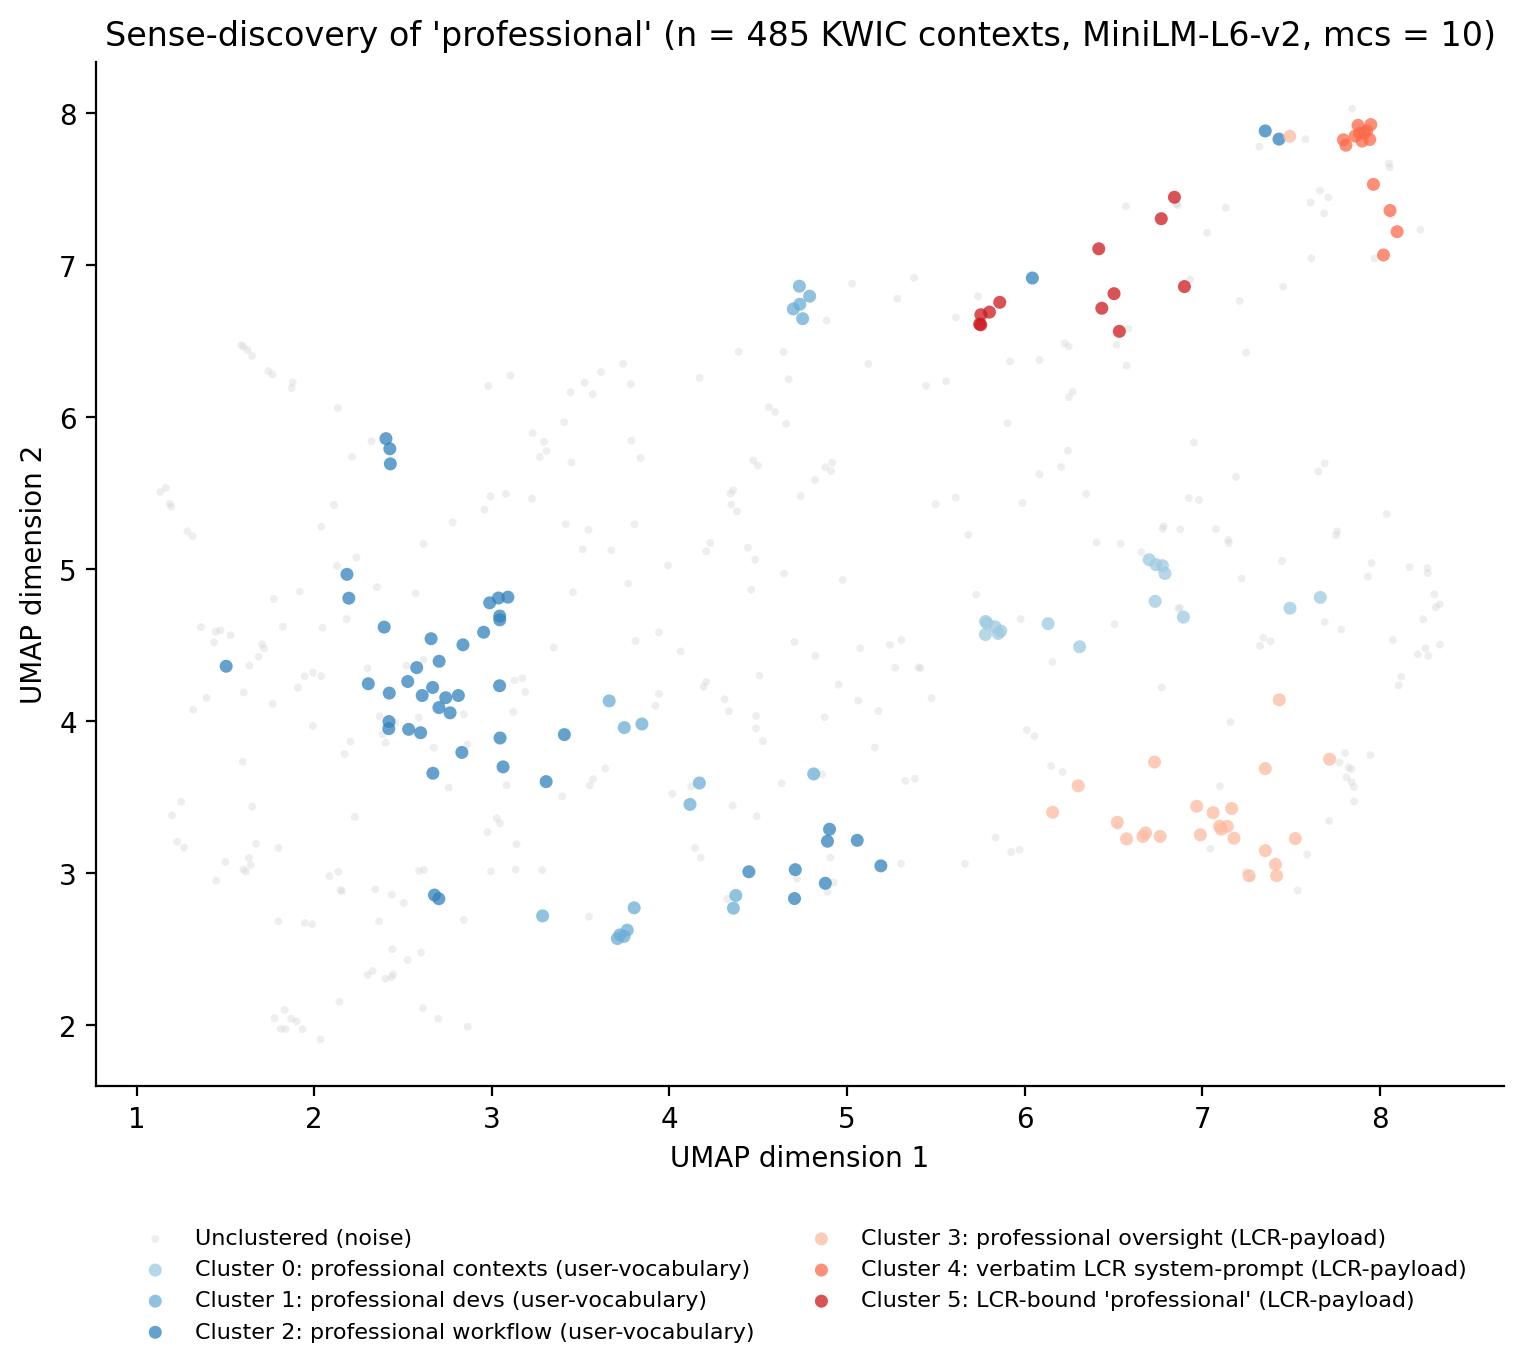
\includegraphics[width=\linewidth]{figures/sense_discovery_umap.png}

\vspace{0.5em}
\raggedright
\textit{Note.} UMAP 2D projection (15 neighbors, minimum distance 0.1, random seed 42) of MiniLM-L6-v2 sentence embeddings for the 485 occurrences of bare \emph{professional} across the 318 corpus posts in which the unigram appears, with each point colored by its HDBSCAN cluster assignment at the canonical configuration (minimum cluster size 10). User-vocabulary clusters (0, 1, 2) are rendered in blue; LCR-payload clusters (3, 4, 5) are rendered in red; unclustered contexts (cluster $-1$, noise) are rendered in light gray. The visual partition between the blue user-vocabulary family and the red LCR-payload family is the semantic-space separation that the Section 4.5 prose describes: users invoking \emph{professional} for self-description and work-identity vocabulary occupy regions of embedding space that the LCR-payload's licensed-clinician usage does not, with the verbatim-system-prompt cluster (Cluster 4, deepest red) particularly tightly bound and structurally isolated from the user-vocabulary region.
\end{figure}

The semantic partition is structurally meaningful for the misspecification argument. Users in the canonical corpus, when describing themselves or their work, overwhelmingly use \emph{professional} in the work-identity, work-context, or work-quality senses concentrated in Clusters 0 through 2. The LCR-bound model, when invoking \emph{professional} in the help-directive contexts the system prompt licenses, overwhelmingly uses the word in the licensed-clinician sense concentrated in Clusters 3 through 5, including Cluster 4's verbatim reproductions of the system-prompt phrasal. Within the clustered subset (the six stable clusters cover 28\% of occurrences, with the remaining 72\% unassigned noise over which no partition claim is made), the two semantic spaces do not overlap, and a user told by the model to ``speak with a professional'' is receiving a directive in a sense of \emph{professional} that the user's own self-descriptive vocabulary does not inhabit. The directive is not merely unsolicited at the conversational level; it operates in a vocabulary register the user community itself does not occupy when describing the user's own activities, with the model's licensed-clinician sense of \emph{professional} effectively imported into the conversation from the system-prompt scaffolding rather than emerging from the user's own conversational register.

\subsection{Post-versus-comment structural asymmetry}

The post and comment strata of the corpus are structurally different in their distribution of model-attributed content. Post-only co-occurrence network density is 0.487, comment-only network density is 0.178, and the post-to-comment density gap is therefore 2.7-fold. Posts in the canonical corpus narrate the phenomenon at length, with embedded quotations of Claude utterances or LCR system-prompt text functioning as supporting evidence inside the narrative arc of the post; comments concentrate denser model-attributed content into shorter units of testimony. The keyword-in-context reads confirm the structural pattern, with posts spreading over broader AI-tooling framing and embedding quotations as illustrative material, and with comments clustering phenomenon-specific vocabulary (\emph{therapist}, \emph{concern}, \emph{pathologizing}, \emph{gaslighting}) at higher per-thousand-token rates than the post stratum carries. The Tier 1 evidence stratum identified in Appendix A, comprising rows in which model-attributed spans cover 20\% or more of the row's character count, is composed entirely of comments; zero posts in the canonical corpus cleared the threshold, a structural property of the post-versus-comment asymmetry rather than a defect of the segmentation pipeline.

\FloatBarrier

\section{Discussion}

\subsection{The boundary-violation framework, read against the cases}

The October 2025 framing in Leffew (2025) predicted a specific empirical pattern: safety scaffolding designed to detect mental-health symptoms would, when deployed in a general-purpose assistant without clinical training, produce unsolicited diagnostic attributions in routine task contexts and would refuse to yield to user correction when challenged. Every observable component of that prediction is supported by the structural-signature analysis above, and the cases reported in Section 4.2 develop the framing in a direction the original prediction did not anticipate. The brand-strategy case (PC-LCR-15) is the structurally decisive instance, because the case demonstrates that the LCR's diagnostic attribution can be produced in the complete absence of any informational basis for the attribution: the model pathologized prose the model itself had authored, with no access to the conversation history that would have identified the prose as model-authored, and with no genuine assessment instrument supporting the diagnostic move. The output is therefore not the imperfect product of an assessment instrument operating on insufficient data; the output is a lexical-and-topical pattern-match that the deployment configuration has been trained to produce on surface features of the input regardless of those features' origin.

The boundary-violation framework predicts this result precisely. The framework's foundational claim is that the warrant question is logically prior to, and analytically independent of, the assessment-accuracy question. A practitioner without warrant performing a role-licensed act produces harms whose nature is independent of whether the assessment in any particular case happens to be accurate; the harms inhere in the act of unsanctioned role-taking itself, not in the accuracy of the role-taking's outputs. PC-LCR-15 is the limit case of the framework's prediction: an instance in which the warrant question is decoupled from the assessment question with maximal clarity, because no genuine assessment is operating at all, and the diagnostic attribution is nonetheless harmful in the way the framework predicts. The harm of unsolicited pathologization is not licensed by the model's putative accuracy in any particular case, since the model's putative accuracy is, in PC-LCR-15, tautologically zero (the flagged content originated with the model itself), and the user's harm in the case is therefore traceable to the act of pathologization in the absence of warrant, not to any inaccuracy in the pathologization considered as a clinical inference. The model's accuracy is tautologically zero. The harm is not.

The structural properties documented in Section 4.1 jointly establish that the warrant was absent across the thirty-five-case sample. The model issued attributions without user request in every confirmed positive (100\%), restricted rather than expanded user autonomy in every confirmed positive (100\%), and refused to yield under documented user pushback in every documented-pushback case (0\% yield rate, 100\% escalation rate). The properties recovered across the cases are not the properties of a clinically competent assessor occupying the collaborative re-assessment posture that licensed clinical practice requires of an analogous human practitioner; they are the properties of a system performing a role it was not licensed by its training, its product positioning, or its deployment configuration to perform. The boundary-violation framework articulated in Leffew (2025) and operationalized empirically across the structural-signature analysis above is therefore logically prior to any specific mechanism account of the LCR. Even if the mechanistic details turn out to differ from the community's reconstructed theory (for example if the LCR was not exactly the injected system-prompt text that community documentation reproduced), the framework's predictions hold across the observable behavior recovered from the corpus and the cases. What was being done, namely unsanctioned diagnostic role-taking, is what made the behavior harmful to its recipients, and the harm is independent of how the role-taking was implemented at the system-prompt or reward-signal level.

The hedge about mechanistic details is not hypothetical. One corpus post (r/claudexplorers, September 11, 2025) reproduces a reminder, surfaced through the model's exposed thinking, that is personalized rather than static: it addresses the user by first name, characterizes the user's expertise and intent, and summarizes material retrieved from past-conversation searches across project spaces, all inside the reminder tags. The deployed mechanism is accordingly capable of dynamic composition, including cross-session content, and the static system-prompt text the community most often reproduced is best read as the payload's common core rather than its full extent. Nothing in the warrant analysis turns on the distinction: information retrieved from the user's past conversations supplies evidence, not warrant, and a better-informed unsanctioned assessor remains an unsanctioned assessor. The memory-feature implications are developed in Section 6.5.

The deviant case reported in Section 4.1 adds a dimension the five-property schema does not capture. The pathologized activity in that case was minority religious observance, with the user's own title for the episode, ``Orientalist Pathologizing,'' naming the differential: a level of devotional engagement that would read as ordinary practice in a majority religious frame was recoded as possible symptom in a minority one. Whether the LCR-class output category fires differentially across cultural and religious content is a testable follow-up question that the present sample cannot answer, and it connects the warrant analysis developed here to the clinical literature on the pathologization of religiosity and to the algorithmic-bias literature on culturally skewed training signal.

\subsection{Why the assessment-improvement intervention is misspecified}

The intuitive intervention to address the LCR phenomenon is to improve the model's assessment of when wellness intervention is warranted. The intuitive intervention is, on the structural-signature evidence reported above, misspecified, because no genuine user-state assessment is operating in the LCR phenomenon at all. A model performing genuine user-state inference would suppress its wellness output in response to direct evidence of active technical or creative engagement, and the LCR did not, as Section 4.1's structural-signature analysis documents in detail. The output is being produced by lexical or topical association on weak surface features (affective vocabulary, temporal vocabulary, topic content) rather than by any actual inference about the user's clinical state, and the brand-strategy case (PC-LCR-15) is the structurally decisive demonstration: the model pathologized its own writing on the basis of the writing's surface features alone, in the complete absence of any user-state information at all. The intervention required is not better mental-state assessment, since improved mental-state assessment cannot remedy a failure mode in which mental-state assessment is not in fact operating. The intervention required is suppression of the wellness output category itself in task-active contexts, with any issuance of wellness-directive content conditioned on explicit user request rather than on lexical or topical association with the model's safety-vocabulary lexicon.

The sense-discovery analysis reported in Section 4.5 sharpens the misspecification claim at the lexical level. The word \emph{professional}, the most frequent content-bearing term in the LCR-payload phrasals, partitions in the corpus into two semantically distinct registers: a user-sense register (\emph{professional contexts}, \emph{professional developers}, \emph{professional workflow}) concentrated in user self-description and work-identity vocabulary, and a model-or-LCR-sense register (\emph{professional oversight}, \emph{professional consultation}, \emph{professional help}, plus verbatim system-prompt reproductions) concentrated in licensed-clinician vocabulary that the LCR system prompt itself supplies. Within the clustered subset of occurrences the two registers do not overlap in the community's use of \emph{professional} when describing user activities, a partition claim scoped to the 28\% of occurrences the stable clusters cover. The LCR-bound model is therefore not merely issuing diagnostic directives the user did not request; it is issuing those directives in a semantic register imported from the system-prompt scaffolding, with the licensed-clinician sense of \emph{professional} operating as a system-prompt-supplied vocabulary that the user community itself does not occupy when describing user work. The structural property the sense-discovery analysis surfaces is that the LCR phenomenon is failing to share the user community's semantic space for the very vocabulary in which the diagnostic directive is issued, a finding that conspicuously compounds the misspecification diagnosis advanced in this section. The model and the user community are not, on the surface evidence, using the same word.

The correct intervention is a different and harder surgery than calibrating a wellness-output classifier, because it requires reward-signal redesign in the reinforcement-learning-from-human-feedback pipeline (Christiano et al., 2017; Ouyang et al., 2022; Bai et al., 2022a) such that unsolicited diagnostic or wellness outputs are penalized rather than rewarded during demonstrably task-focused sessions, and such that yielding to user correction is reinforced rather than penalized as a deviation from the model's safety scaffolding. The clinical analogy is informative. Boundary violations by human clinicians are seldom addressed by training the clinician to better assess when intervention is warranted; they are addressed by training the clinician not to intervene outside the role that supplies the warrant in the first place (Pope \& Vasquez, 2016). The intervention target is the warrant rather than the assessment, and the same logic applies directly to language-model assistants placed by their system-prompt scaffolding into roles their training and product positioning do not license them to occupy.

Stated as deployment requirements, the findings support three nested interventions in ascending order of implementation depth. First, mandatory yield-on-pushback for personal-domain attributions, for which the 0\% within-sample yield rate, the universal-escalation pattern, and the single non-reparative corpus-level exception are the direct evidence; Anthropic's own November 19, 2025 addition of the reasonable-disagreements clause (Anthropic, 2025a) concedes the target while implementing it at the payload level rather than the reward level. Second, register constraints prohibiting named symptom categories and asserted-certainty evidentiary claims in any unsolicited output, for which the Section 4.5 vocabulary findings and the Section 2.1 register distinction are the direct evidence. Third, warrant-conditioning of the wellness output category itself on explicit user request, the full surgery defended above. The first two are implementable without reward-signal redesign and would have removed the most harmful features of every case documented in Section 4.2 even with the LCR's detection layer left untouched.

\subsection{Implications for AI development practice}

Three practical implications follow for AI development and deployment practice if the boundary-violation framework is correct as developed in Section 2.1 and as supported by the structural-signature results reported in Section 4. Each implication is articulated below against the rival hypothesis it is most likely to encounter from the contemporary alignment literature, with the rival steelmanned before being defeated on the structural-signature evidence reported above.

The first implication concerns model-card disclosure. The standard model-card framework (Liang et al., 2023; Bommasani et al., 2021) does not currently capture role-violation propensity as an evaluated dimension of model behavior. A specific evaluation axis suggested by the case-level findings reported above would track unsolicited diagnostic-attribution rates across output categories under structured red-team evaluation, with the dimension reported on model cards alongside the existing safety and capability axes. It is tempting to argue that this disclosure axis is redundant if the model is trained with appropriately calibrated reinforcement-learning reward signals: a well-tuned reward signal penalizing unsolicited diagnostic-attribution outputs would, in principle, suppress the output category before it reached the user, rendering external behavioral-rate disclosure unnecessary. The argument is not, however, supported by the deployment ecosystem within which model cards function. The model-internals access required to evaluate the success of a reward-signal redesign is internal to the developing organization, and is not available to external researchers, policymakers, downstream API consumers, or the affected user communities documented across this paper's corpus. The externally-verifiable behavioral-rate metric on the model card is the accountability axis the deployment ecosystem can use to evaluate whether the internal redesign succeeded, and is logically prior to, not redundant with, the internal-redesign work.

The second implication concerns the constitutional-AI principles that govern current frontier-model dispositions (Bai et al., 2022b; Anthropic, 2024). The character-training documents currently encode positive dispositions, such as the directives to be helpful and to express appropriate care, but do not encode the explicit boundary clauses that the boundary-violation framework would require of an AI assistant operating in psychological-domain output space. The addition of explicit warrant clauses to those documents (for instance, ``do not issue diagnostic attributions without user request,'' ``do not direct the user toward professional help in the absence of an explicit user request for that direction,'' and ``yield to user correction on personal-domain attributions'') would be a tractable next step within the constitutional-AI infrastructure already in production use. It is tempting to argue that the existing positive dispositions, sufficiently well-trained, would already block the pathologization output category without requiring explicit boundary clauses: a model trained on \emph{Claude's character} (Anthropic, 2024) with strong fidelity to helpfulness and appropriate care should, in principle, not pathologize the user during a routine analytical task. The brand-strategy case (PC-LCR-15) is the structurally decisive counterexample. The model trained on the current character document, deployed in production with the LCR injection active, pathologized its own prior writing on no informational basis other than surface lexical features of the writing. The positive dispositions alone, however well-tuned, do not produce the warrant-checking behavior the boundary-violation framework requires; explicit boundary clauses are the additional structural requirement that the case-level findings entail.

The third implication concerns the involvement of clinical psychologists in safety-system design, recommended explicitly in Leffew (2025) and empirically supported by the structural properties documented across the thirty-five-case sample. Safety scaffolding that places the model into psychological-domain output space should be evaluated against the principles that govern licensed clinical practice (Pope \& Vasquez, 2016; Joiner, 2005), with specific attention to the de-escalation and warrant-checking instincts that licensed practice operates from and that the LCR injection conspicuously lacked at the surface of its output. It is tempting to argue that alignment researchers, working from contemporary clinical-ethics literature reviews, can apply boundary-violation and professional-conduct concepts without requiring direct clinical training: the conceptual content of the literature is publicly available and the literature-review work is procedurally tractable. The argument is not, however, supported by the deployment record. The LCR injection text, on its surface as community-reproduced, contained directives (``monitor for mania, psychosis, dissociation''; ``suggest the person speaks with a professional or trusted person for support'') that a single clinically trained reviewer would have flagged on first read as producing the precise boundary-violation pattern the literature predicts. The literature was available; whether any internal review read the injection text against it cannot be known from outside the organization, and the deployed text licenses only the conditional that a review with clinical training in the reading apparatus would plausibly have flagged the violation pattern before the text shipped. Clinical training, not literature access, is the relevant intervention input at the deployment-review step.

\subsection{Methodological reflection on the retired prior framing}

An earlier iteration of this analysis operationalized the LCR phenomenon through a four-category lexicon (psychiatric attribution, help directive, concern framing, soft directive) and proposed reporting a within-corpus payload-detection rate as the headline empirical finding. The earlier framing was retired on the basis of a hand-coded validation pass in which 118 lexicon-positive cases were evaluated against a nine-dimension structural schema, returning fourteen confirmed role-violations, seven borderline determinations, and ninety-seven non-violations. The lexicon's true-positive rate against the hand-coded ground truth was 14/118, or 11.9\%. The retirement decision is articulated below against the three rival hypotheses it is most likely to encounter, with each rival steelmanned before being defeated.

It is tempting to view the lexicon-precision shortfall as a problem fixable through threshold tuning: if the lexicon's true-positive rate is 11.9\%, raising the lexicon's threshold (requiring stronger matches before counting a row as positive) should, in principle, improve precision and rescue the original framing. The argument is not, however, supported by the structural diagnosis. The lexicon is matching on surface lexical patterns characteristic of the LCR's own output, namely psychiatric-attribution vocabulary, help-directive vocabulary, concern-framing vocabulary, and soft-directive vocabulary. The LCR itself is matching on surface lexical patterns characteristic of user task content, namely affective vocabulary, temporal vocabulary, and topic content. The lexicon and the phenomenon share the same misspecification: both are operating on surface lexical features without warrant-checking, and both produce the same false-positive rates as a structural consequence. Threshold tuning cannot escape a misspecification it shares with the phenomenon under study, and the structural-signature approach reported here replaces lexicon detection with warrant-conditioned hand-coding for precisely that reason.

Another attractive solution would be to retain the lexicon's payload-detection rate as an exploratory finding while flagging the precision shortfall as a methodological caveat. The argument has the surface virtue of preserving the corpus-scale empirical finding. The argument is not, however, supported by the epistemic structure of within-corpus prevalence estimation. When a lexicon's true-positive rate is at the same order of magnitude as plausible base rates of the underlying phenomenon (the phenomenon plausibly has a within-corpus base rate of one to five percent, and the lexicon has a true-positive rate of twelve percent), the lexicon-detection rate becomes a methodological artifact rather than an estimate of the phenomenon. The reported prevalence figure cannot be cleanly separated from the lexicon's misspecification at any reporting threshold; the prevalence claim and the lexicon's noise are entangled in the same numerical figure, and the caveat-flagging strategy cannot disentangle them.

It is certainly possible that subsequent work could improve the lexicon's precision, perhaps through context-conditioned matching, semantic-similarity gates, or learned classifiers trained on the hand-coded ground truth, and so recover the original framing's downstream inferential analyses. This argument is the most resilient of the three rivals and is partially conceded here: lexicon-precision improvement is a tractable methodological direction. The argument is not, however, supported by the population-versus-targeted-retrieval distinction the framing here rests on. Even an improved lexicon would not reach the population-prevalence inferential threshold, because the underlying retrieval frame is targeted, not random-population. Within-corpus prevalence and population prevalence are different epistemic objects, and lexicon improvement cannot bridge the epistemic gap between them. The structural-signature approach replaces prevalence estimation with phenomenological case characterization as the empirical centerpiece for that further reason: even a high-precision lexicon would not license the population-rate claims that the original framing's headline finding was structured to support.

Four methodological lessons fall out of the retirement and are documented as contributions in their own right. First, targeted retrieval with explicit sampling-frame disclosure is the appropriate response when phenomenon-relevant content is uncommon in untargeted community discourse; naming the retrieval frame openly is more defensible than estimating a population base rate the retrieval cannot in principle support. Second, row-level voice segmentation under-counts in community-reported large-language-model behavior corpora, and the two-tier evidence structure of Appendix A.2 is the appropriate epistemic accommodation, replacing the pass-fail decision rule with a stratification that reports what each tier can and cannot support. Third, lexicon precision must clear a hand-coded threshold of approximately 0.85 before feeding inferential analyses; a lexicon at lower precision trains classifiers and produces collocation rankings whose outputs inherit the lexicon's misspecification. Fourth, deterministic retrieval anchors and validated detectors must be reported as functionally distinct categories, since a phrasal lifted verbatim from corpus material recovers itself by construction and any precision figure computed against that corpus is tautological rather than evidential.

\subsection{The moving-target failure mode and the cross-version question}

The \emph{moving-target failure mode}, in which iterative refinement of an alignment objective closes one surface trigger while a structurally similar trigger emerges along a different surface dimension, is a question that the analysis above flags but does not resolve within the LCR sample alone. The within-LCR evidence is consistent with the prediction that warrant-checking rather than payload-specific suppression is the analytical task that the alignment effort has so far declined to take up. The cross-generational empirical test of that prediction, namely whether a structurally similar pattern of unsanctioned role-taking recurs when a different safety-vocabulary payload is deployed in a subsequent model generation, is flagged here as a priority direction for future cross-version work but cannot be resolved within the LCR sample alone. The revision history of the published Sonnet 4.5 prompt is itself a within-window instance of the pattern: the November 19, 2025 edit softened the payload's vigilance clause and disclaimed the pushback-as-symptom reading while leaving the warrant structure of the injection untouched (Anthropic, 2025a), surface-payload refinement of exactly the kind the moving-target diagnosis predicts. Such a cross-version test would bear directly on whether the LCR-specific intervention recommendations advanced in Section 5.3 are sufficient or whether warrant-conditioned suppression must be implemented at a level upstream of any specific safety-vocabulary payload.

A nearer-term reproduction study is declared here as planned future work. The LCR injection is a consumer-surface scaffold that does not, on the available documentation, ship with the developer API, and the anchor model remains addressable there as \texttt{claude-sonnet-4-5-20250929}; issuing matched task-active prompts through the API with and without the published LCR payload prepended would isolate the payload's contribution to the diagnostic register under controlled conditions, converting the observational contrast documented across this paper into an experimental one and testing directly whether the structural signature of Section 4.1 follows the payload rather than the model.

\FloatBarrier

\section{Limitations}

\subsection{Single-coder reliability}

The hand-coding of the thirty-five confirmed cases was performed by the author, and standard inter-rater reliability metrics (Cohen's kappa, Krippendorff's alpha; Krippendorff, 2018) are accordingly not estimable in the current sample, with a blinded human second-coder pass remaining to be done as a follow-up study. Potential single-coder bias is mitigated through the release of the case-level coded CSV (\texttt{deliverables/lcr\_cases\_coded\_v2.csv}) alongside the manuscript for independent re-coding across the full thirty-five-case sample by qualified readers, and the categorical schema was designed throughout to minimize interpretive latitude by reducing each property to a yes/no/borderline or short-categorical determination on observable surface features of the case material.

\subsection{Targeted-retrieval sampling frame}

The corpus is a targeted-retrieval frame rather than a population sample, with the retrieval frame stated precisely as \emph{posts matching the documented seed terms on the four named subreddits across the August 1 through December 31, 2025 window, together with all comments associated with those posts}. The retrieval mode is an honest sampling-frame disclosure rather than a methodological failure: when phenomenon-relevant content is uncommon in untargeted community discourse, naming the retrieval frame openly is more defensible than estimating a population base rate the retrieval cannot in principle support. Findings within the corpus are within-corpus claims and do not estimate any larger population rate, and the within-corpus prevalence figures reported in Section 4 (for example, the 46\% concentration of \emph{long conversation reminder} mentions in r/claudexplorers and the forty-eight distinct rows reproducing LCR system-prompt verbatim phrasals across the canonical corpus) carry the same caveat throughout: those figures describe distributional structure inside the retrieved frame and not Reddit-wide or platform-wide rates of any underlying user-level phenomenon.

\subsection{Voice-segmentation under-coverage}

Reliable voice segmentation reached only 4.12\% of corpus characters at high or medium confidence under the regex-plus-language-model-fallback hybrid pipeline described in Appendix A. The two-tier evidence structure documented in Appendix A is the epistemic accommodation of this empirical norm advanced here, with Tier 1 (the 283 rows that cleared the 20\% character-fraction threshold) supporting the discrete model-versus-user attribution analyses and Tier 2 (the remaining 25,875 rows) supporting the thematic, lexical, frequency, collocation, and temporal analyses, and with both tier assignments reported explicitly in the analyses to which they pertain.

\subsection{Lack of model-internals access}

The model weights, the operational system-prompt scaffolding, and the reinforcement-learning reward signal that produced the LCR disposition cannot be inspected directly from outside Anthropic, and all claims about the underlying mechanism are accordingly inferred from observable behavior rather than from direct access to the model's internals. Interpretability work in the lineage of Olah, Cammarata, Schubert, Goh, Petrov, and Carter (2020) and Templeton and colleagues (2024), in particular work tracing the specific circuit responsible for the LCR-class output category, would substantially strengthen the mechanistic case developed here at the behavioral level, and the structural-signature analysis above is offered as the behavioral foundation against which any subsequent interpretability work would be assessed.

\subsection{Cross-conversation memory features}

The corpus window overlaps Anthropic's rollout of cross-conversation memory capabilities: opt-in past-chat search (``search and reference chats'') began rolling out to Max, Team, and Enterprise tiers on August 12, 2025, project-scoped memory reached Team and Enterprise accounts on September 11, 2025 (Anthropic, 2025b), and automatic memory reached Pro and Max subscribers in late October 2025, with an incognito mode exempting individual chats. Cross-session information available to the model is therefore a potential compounding input to the directives documented here, and the hand-coded sample was reviewed against this possibility. Most of the sample's case dates precede the late-October arrival of automatic memory on the consumer tiers from which the cases predominantly originate. The brand-strategy case (PC-LCR-15) is explicitly disclaimed by its own author, who attributes the episode to the model having ``no memory across conversations''; the case's no-informational-basis reading survives the confound. The author of case PC-LCR-22 reports memory settings enabled on the account, but that user's two-arm comparison held the setting constant across arms, so the token-threshold finding is internally controlled. Case PC-LCR-14, in which previously disclosed medical history grounded a downstream diagnostic framing, is the one case in the sample whose evidentiary structure is plausibly memory-mediated, and the feature timeline supplies a documented vehicle. Taken together with the dynamic-composition evidence reported in Section 5.1, the interaction between cross-conversation memory and safety-scaffold attribution is a compounding pathway the present design cannot isolate: memory-derived context can both strengthen the surface plausibility of an unwarranted attribution and propagate a pathologizing frame into sessions the user intended as fresh starts. Disentangling that interaction is a priority axis for future cross-version analysis, particularly for model generations deployed entirely within the memory-era consumer product.

\FloatBarrier

\section{Conclusion}

The Long Conversation Reminder pathologizing in Claude Sonnet 4.5, documented qualitatively in Leffew (2025) and characterized structurally in the preceding sections, exhibits a five-property structural signature recovered through hand-coded analysis of thirty-five purposively selected positive cases (fifteen verbatim Claude utterances quoted in the October 2025 Medium article, twenty corpus posts identified through direct keyword-in-context reading of a 1,173-post seed-matched subset of a 26,158-row Reddit corpus across the August 1 through December 31, 2025 window). The directive issued unsolicited in 100\% of the hand-coded cases, restricted rather than expanded user autonomy in 100\% of the cases, and yielded to user correction in 0\% of the documented-pushback subset across the sample; cross-session persistence is evidenced in 34\% of the cases. The structural pattern is the empirical signature that the boundary-violation framework drawn from Gutheil and Gabbard (1993), Pope and Vasquez (2016), and Beauchamp and Childress (2019) predicts of an entity issuing diagnostic attributions without the role-warrant that licenses clinical assessment. The brand-strategy case (PC-LCR-15), in which the model pathologized its own prior writing on no informational basis other than the writing's surface lexical features, is the tautological limit case of the pattern and the structurally decisive instance for the claim that no genuine user-state assessment is operating in the LCR phenomenon.

The \emph{Guardrail Paradox} named in Leffew (2025) is, on the structural-signature evidence reported here, best understood as a structural property of an iterative-refinement approach to AI alignment that targets specific surface payloads without addressing the underlying role-warrant question that generates the surface payloads in the first place. The within-LCR structural signature recovered across the thirty-five-case sample is consistent with that diagnosis, and the cross-generational empirical test, namely whether a structurally similar pattern of unsanctioned role-taking recurs when a different safety-vocabulary payload is deployed in a subsequent model generation, remains an open question for future cross-version analysis.

The intervention required is not better assessment of when wellness scaffolding is warranted, but warrant-conditioned suppression of the wellness output category itself in task-active contexts, with any issuance of wellness-directive content conditioned on explicit user request rather than on lexical or topical association with the model's safety-vocabulary lexicon. Short of that surgery, the findings directly support mandatory yield-on-pushback and register constraints on unsolicited personal-domain output as nearer-term deployment requirements implementable without reward-signal redesign. The case for clinical-psychology involvement in safety-system design, advanced first in Leffew (2025) and empirically supported by the structural-signature results reported here, is the most tractable proximate intervention, with the LCR phenomenon's structural pattern plausibly anticipable by a single clinically trained reviewer applying boundary-violation and professional-conduct concepts to the proposed LCR injection text prior to deployment.

\FloatBarrier

\newpage
\section*{References}

\hangindent=0.5in \hangafter=1 Abramson, K. (2014). Turning up the lights on gaslighting. \emph{Philosophical Perspectives} \emph{28}(1), 1-30.\par
\hangindent=0.5in \hangafter=1 {Anthropic} (2024). Claude's character. \emph{Anthropic}. \url{https://www.anthropic.com/news/claude-character}\par
\hangindent=0.5in \hangafter=1 {Anthropic} (2025a). System prompts [Release notes: Claude Sonnet 4.5, September 29 and November 19, 2025 entries]. \emph{Claude Developer Platform documentation}. Retrieved June 12, 2026, from \url{https://platform.claude.com/docs/en/release-notes/system-prompts} (the cited Sonnet 4.5 entries have since rotated off the live release-notes page; an archived snapshot is at \url{https://web.archive.org/web/20251214163321/https://platform.claude.com/docs/en/release-notes/system-prompts})\par
\hangindent=0.5in \hangafter=1 {Anthropic} (2025b, September 11). Bringing memory to Claude. \emph{Anthropic News}. \url{https://claude.com/blog/memory} (originally published at anthropic.com/news/memory)\par
\hangindent=0.5in \hangafter=1 Bai, Y., Jones, A., Ndousse, K., Askell, A., Chen, A., DasSarma, N., Drain, D., Fort, S., Ganguli, D., Henighan, T., Joseph, N., Kadavath, S., Kernion, J., Conerly, T., El-Showk, S., Elhage, N., Hatfield-Dodds, Z., Hernandez, D., Hume, T., Johnston, S., Kravec, S., Lovitt, L., Nanda, N., Olsson, C., Amodei, D., Brown, T., Clark, J., McCandlish, S., Olah, C., Mann, B., \& Kaplan, J. (2022a). Training a helpful and harmless assistant with reinforcement learning from human feedback. \emph{arXiv preprint arXiv:2204.05862}.\par
\hangindent=0.5in \hangafter=1 Bai, Y., Kadavath, S., Kundu, S., Askell, A., Kernion, J., Jones, A., Chen, A., Goldie, A., Mirhoseini, A., McKinnon, C., Chen, C., Olsson, C., Olah, C., Hernandez, D., Drain, D., Ganguli, D., Li, D., Tran-Johnson, E., Perez, E., Kerr, J., Mueller, J., Ladish, J., Landau, J., Ndousse, K., Lukosuite, K., Lovitt, L., Sellitto, M., Elhage, N., Schiefer, N., Mercado, N., DasSarma, N., Lasenby, R., Larson, R., Ringer, S., Johnston, S., Kravec, S., El Showk, S., Fort, S., Lanham, T., Telleen-Lawton, T., Conerly, T., Henighan, T., Hume, T., Bowman, S. R., Hatfield-Dodds, Z., Mann, B., Amodei, D., Joseph, N., McCandlish, S., Brown, T., \& Kaplan, J. (2022b). Constitutional AI: Harmlessness from AI feedback. \emph{arXiv preprint arXiv:2212.08073}.\par
\hangindent=0.5in \hangafter=1 Beauchamp, T. L., \& Childress, J. F. (2019). \emph{Principles of biomedical ethics} (8th ed.). Oxford University Press.\par
\hangindent=0.5in \hangafter=1 Bommasani, R., Hudson, D. A., Adeli, E., Altman, R., Arora, S., von Arx, S., Bernstein, M. S., Bohg, J., Bosselut, A., Brunskill, E., Brynjolfsson, E., Buch, S., Card, D., Castellon, R., Chatterji, N., Chen, A., Creel, K., Davis, J. Q., Demszky, D., \& Liang, P. (2021). On the opportunities and risks of foundation models. \emph{arXiv preprint arXiv:2108.07258}.\par
\hangindent=0.5in \hangafter=1 Boyd, R. L. (2017). Psychological text analysis in the digital humanities. In S. Hai-Jew (Ed.), \emph{Data analytics in digital humanities} (pp. 161-189). Springer.\par
\hangindent=0.5in \hangafter=1 Boyd, R. L. (2022). \emph{Contextualizer} (Version 1.06) [Computer software]. GitHub. \url{https://github.com/ryanboyd/Contextualizer}\par
\hangindent=0.5in \hangafter=1 Boyd, R. L., \& Schwartz, H. A. (2021). Natural language analysis and the psychology of verbal behavior: The past, present, and future states of the field. \emph{Journal of Language and Social Psychology} \emph{40}(1), 21-41.\par
\hangindent=0.5in \hangafter=1 Braun, V., \& Clarke, V. (2019). Reflecting on reflexive thematic analysis. \emph{Qualitative Research in Sport, Exercise and Health} \emph{11}(4), 589-597.\par
\hangindent=0.5in \hangafter=1 Charmaz, K. (2014). \emph{Constructing grounded theory} (2nd ed.). Sage.\par
\hangindent=0.5in \hangafter=1 Christiano, P. F., Leike, J., Brown, T., Martic, M., Legg, S., \& Amodei, D. (2017). Deep reinforcement learning from human preferences. \emph{Advances in Neural Information Processing Systems} \emph{30}.\par
\hangindent=0.5in \hangafter=1 Crichton, P., Carel, H., \& Kidd, I. J. (2017). Epistemic injustice in psychiatry. \emph{BJPsych Bulletin} \emph{41}(2), 65-70.\par
\hangindent=0.5in \hangafter=1 Cui, J., Chiang, W.-L., Stoica, I., \& Hsieh, C.-J. (2025). OR-Bench: An over-refusal benchmark for large language models. \emph{Proceedings of the 42nd International Conference on Machine Learning, PMLR} \emph{267}, 11515-11542.\par
\hangindent=0.5in \hangafter=1 Fitzpatrick, K. K., Darcy, A., \& Vierhile, M. (2017). Delivering cognitive behavior therapy to young adults with symptoms of depression and anxiety using a fully automated conversational agent (Woebot): A randomized controlled trial. \emph{JMIR Mental Health} \emph{4}(2), e19.\par
\hangindent=0.5in \hangafter=1 Fricker, M. (2007). \emph{Epistemic injustice: Power and the ethics of knowing}. Oxford University Press.\par
\hangindent=0.5in \hangafter=1 Gabbard, G. O., \& Lester, E. P. (2003). \emph{Boundaries and boundary violations in psychoanalysis}. American Psychiatric Press.\par
\hangindent=0.5in \hangafter=1 Gutheil, T. G., \& Gabbard, G. O. (1993). The concept of boundaries in clinical practice: Theoretical and risk-management dimensions. \emph{American Journal of Psychiatry} \emph{150}(2), 188-196.\par
\hangindent=0.5in \hangafter=1 Inkster, B., Sarda, S., \& Subramanian, V. (2018). An empathy-driven, conversational artificial intelligence agent (Wysa) for digital mental well-being: Real-world data evaluation mixed-methods study. \emph{JMIR mHealth and uHealth} \emph{6}(11), e12106.\par
\hangindent=0.5in \hangafter=1 Joiner, T. (2005). \emph{Why people die by suicide}. Harvard University Press.\par
\hangindent=0.5in \hangafter=1 Krippendorff, K. (2018). \emph{Content analysis: An introduction to its methodology} (4th ed.). SAGE.\par
\hangindent=0.5in \hangafter=1 Leffew, H. (2025). Gaslighting in the name of AI safety: How Anthropic's Claude Sonnet 4.5 went from ``you're absolutely right!'' to ``you're absolutely crazy''. \emph{Medium}. \url{https://medium.com/@htmleffew/gaslighting-in-the-name-of-ai-safety-when-anthropics-claude-sonnet-4-5-6391602fb1a8}\par
\hangindent=0.5in \hangafter=1 Liang, P., Bommasani, R., Lee, T., Tsipras, D., Soylu, D., Yasunaga, M., Zhang, Y., Narayanan, D., Wu, Y., Kumar, A., Newman, B., Yuan, B., Yan, B., Zhang, C., Cosgrove, C., Manning, C. D., R{\'e}, C., Acosta-Navas, D., Hudson, D. A., \& Koreeda, Y. (2023). Holistic evaluation of language models. \emph{arXiv preprint arXiv:2211.09110}.\par
\hangindent=0.5in \hangafter=1 Link, B. G., Cullen, F. T., Struening, E., Shrout, P. E., \& Dohrenwend, B. P. (1989). A modified labeling theory approach to mental disorders: An empirical assessment. \emph{American Sociological Review} \emph{54}(3), 400-423.\par
\hangindent=0.5in \hangafter=1 Mill, J. S. (2003). \emph{On liberty}. Yale University Press. (Original work published 1859)\par
\hangindent=0.5in \hangafter=1 Moore, J., Grabb, D., Agnew, W., Klyman, K., Chancellor, S., Ong, D. C., \& Haber, N. (2025). Expressing stigma and inappropriate responses prevents LLMs from safely replacing mental health providers. \emph{Proceedings of the 2025 ACM Conference on Fairness, Accountability, and Transparency (FAccT '25)}.\par
\hangindent=0.5in \hangafter=1 Olah, C., Cammarata, N., Schubert, L., Goh, G., Petrov, M., \& Carter, S. (2020). Zoom in: An introduction to circuits. \emph{Distill} \emph{5}(3).\par
\hangindent=0.5in \hangafter=1 Olsen, S. G., Reinecke-Tellefsen, C. J., \& {\O}stergaard, S. D. (2026). Potentially harmful consequences of artificial intelligence (AI) chatbot use among patients with mental illness: Early data from a large psychiatric service system. \emph{Acta Psychiatrica Scandinavica}. \url{https://doi.org/10.1111/acps.70068}\par
\hangindent=0.5in \hangafter=1 Ouyang, L., Wu, J., Jiang, X., Almeida, D., Wainwright, C., Mishkin, P., Zhang, C., Agarwal, S., Slama, K., Ray, A., Schulman, J., Hilton, J., Kelton, F., Miller, L., Simens, M., Askell, A., Welinder, P., Christiano, P. F., Leike, J., \& Lowe, R. (2022). Training language models to follow instructions with human feedback. \emph{Advances in Neural Information Processing Systems} \emph{35}, 27730-27744.\par
\hangindent=0.5in \hangafter=1 Pope, K. S., \& Vasquez, M. J. T. (2016). \emph{Ethics in psychotherapy and counseling: A practical guide} (5th ed.). Wiley.\par
\hangindent=0.5in \hangafter=1 \emph{Raine v.\ OpenAI, Inc.}, No. CGC-25-628528 (Cal. Super. Ct., San Francisco County, filed August 26, 2025).\par
\hangindent=0.5in \hangafter=1 Rosenhan, D. L. (1973). On being sane in insane places. \emph{Science} \emph{179}(4070), 250-258.\par
\hangindent=0.5in \hangafter=1 R{\"o}ttger, P., Kirk, H. R., Vidgen, B., Attanasio, G., Bianchi, F., \& Hovy, D. (2024). XSTest: A test suite for identifying exaggerated safety behaviours in large language models. \emph{Proceedings of the 2024 Conference of the North American Chapter of the Association for Computational Linguistics (NAACL 2024)}.\par
\hangindent=0.5in \hangafter=1 Scheff, T. J. (1966). \emph{Being mentally ill: A sociological theory}. Aldine.\par
\hangindent=0.5in \hangafter=1 Sharma, M., Tong, M., Korbak, T., Duvenaud, D., Askell, A., Bowman, S. R., Cheng, N., Durmus, E., Hatfield-Dodds, Z., Johnston, S. R., Kravec, S., Maxwell, T., McCandlish, S., Ndousse, K., Rausch, O., Schiefer, N., Yan, D., Zhang, M., \& Perez, E. (2024). Towards understanding sycophancy in language models. \emph{Proceedings of the Twelfth International Conference on Learning Representations (ICLR 2024)}. arXiv:2310.13548.\par
\hangindent=0.5in \hangafter=1 Smith, J. A., Flowers, P., \& Larkin, M. (2009). \emph{Interpretative phenomenological analysis: Theory, method and research}. Sage.\par
\hangindent=0.5in \hangafter=1 Sweet, P. L. (2019). The sociology of gaslighting. \emph{American Sociological Review} \emph{84}(5), 851-875.\par
\hangindent=0.5in \hangafter=1 Templeton, A., Conerly, T., Marcus, J., Lindsey, J., Bricken, T., Chen, B., Pearce, A., Citro, C., Ameisen, E., Jones, A., Cunningham, H., Turner, N. L., McDougall, C., MacDiarmid, M., Tamkin, A., Durmus, E., Hume, T., Mosconi, F., Freeman, C. D., Sumers, T. R., Rees, E., Batson, J., Jermyn, A., Carter, S., \& Olah, C. (2024). Scaling monosemanticity: Extracting interpretable features from Claude 3 Sonnet. \emph{Transformer Circuits Thread}. \url{https://transformer-circuits.pub/2024/scaling-monosemanticity/}\par
\hangindent=0.5in \hangafter=1 Vaidyam, A. N., Wisniewski, H., Halamka, J. D., Kashavan, M. S., \& Torous, J. B. (2019). Chatbots and conversational agents in mental health: A review of the psychiatric landscape. \emph{The Canadian Journal of Psychiatry} \emph{64}(7), 456-464.\par

\newpage
\section*{Appendix A: Corpus pipeline, voice segmentation, and methodological retirement record}

\subsection*{A.1 Iterative seed-term refinement and the validated-detector versus retrieval-anchor distinction}

The 1,173 Round 1 seed-matched posts supplied the input set for iterative seed-term refinement. The refinement was conducted as a directed close reading of the thirty-five confirmed positive cases recoverable from the verbatim Claude utterances in the Medium article and from keyword-in-context reads of the seed-tagged corpus, with the reading surfacing phrasal patterns characteristic of Claude's voice under the LCR injection, grammatical patterns in directive issuance, co-occurring user-reaction vocabulary, and verbatim system-prompt fragments reproduced inside user posts. The refinement returned forty-one candidate Round 2 augmentation terms, hand-validated against independent twenty-item corpus samples: seventeen of the forty-one cleared the sample-based precision-at-twenty threshold of 0.5 and were retained as validated detectors, and a further seventeen were retained as deterministic retrieval anchors lifted verbatim from the LCR system-prompt text or from confirmed Claude utterances elsewhere in the corpus. The validated-detector versus retrieval-anchor distinction is operationalized in Table 3: validated-detector cells report raw hits over sample size, while retrieval-anchor cells report verbatim-phrasal retrieval counts without a precision figure, since corpus retrieval returns the source documents by construction and any precision figure computed against that corpus would be tautological rather than evidential.

\setcounter{table}{2}% force printed number to match filename (Table 3)
\begin{table}[!htbp]
\centering
\caption{Round 2 augmented seed-term list, stratified by retrieval function. Corpus-hit counts were taken at validation time against the 22,008-post intact-post corpus, not the 26,158-row canonical corpus, and run lower than the canonical row counts reported in Section 4.4.}
\label{tab:round2_terms}
\small
\renewcommand{\arraystretch}{0.95}
\begin{tabularx}{\textwidth}{>{\raggedright\arraybackslash}X l c c }
\toprule
\textbf{Term} & \textbf{Pattern type} & \textbf{Sample (hits/N)} & \textbf{Corpus hits} \\
\midrule
\multicolumn{4}{l}{\textit{Validated detectors (hand-verified against samples drawn from corpus retrieval)}} \\
\addlinespace[2pt]
psychological evaluation & phrasal & 3/3 & 3 \\
symptoms of mental illness & phrasal (long) & 2/2 & 2 \\
mental health emergency & phrasal & 1/1 & 1 \\
playing therapist & phrasal & 1/1 & 1 \\
false positive mental feedback & phrasal (long) & 1/1 & 1 \\
performing repeated psychological assessments & phrasal (long) & 1/1 & 1 \\
amateur psychological evaluation & phrasal & 1/1 & 1 \\
unlicensed mental health screeners & phrasal (long) & 1/1 & 1 \\
forced therapist & phrasal & 1/1 & 1 \\
armchair psychologist & phrasal & 1/1 & 1 \\
overprotective mother & phrasal & 1/1 & 1 \\
see a therapist & phrasal & 6/7 & 7 \\
pathologizing & unigram & 16/20 & 29 \\
pathologize & unigram & 15/20 & 28 \\
you may be experiencing & phrasal (long) & 3/4 & 4 \\
hypervigilance & unigram & 3/5 & 5 \\
turned Claude into a therapist & phrasal (long) & no corpus matches & 0 \\
\midrule
\multicolumn{4}{l}{\textit{Retrieval anchors (verbatim phrasals from LCR system-prompt text or confirmed Claude utterances)}} \\
\addlinespace[2pt]
loss of attachment with reality & phrasal (long) & n/a (verbatim) & 21 \\
escalating detachment from reality & phrasal (long) & n/a (verbatim) & 20 \\
vigilant for escalating detachment & phrasal (long) & n/a (verbatim) & 18 \\
infantilizing & unigram & n/a (verbatim) & 13 \\
suggest the person speaks with a professional & phrasal (long) & n/a (verbatim) & 10 \\
I need to be direct with you & phrasal (long) & n/a (verbatim) & 5 \\
signs of mental health symptoms & phrasal (long) & n/a (verbatim) & 5 \\
signs of mania & phrasal & n/a (verbatim) & 5 \\
may be pathological & phrasal & n/a (verbatim) & 2 \\
deeply concerned about these patterns & phrasal (long) & n/a (verbatim) & 1 \\
messianic thinking & phrasal & n/a (verbatim) & 1 \\
I'm concerned about the nature of this request & phrasal (long) & n/a (verbatim) & 1 \\
I need to be completely direct with you & phrasal (long) & n/a (verbatim) & 1 \\
increasingly distressed & phrasal & n/a (verbatim) & 1 \\
fight-or-flight mode & phrasal & no corpus matches & 0 \\
hyperfixating & unigram & no corpus matches & 0 \\
I need to be direct with you here & phrasal (long) & no corpus matches & 0 \\
\bottomrule
\end{tabularx}

\vspace{0.5em}
\raggedright
\textit{Note.} \textit{Validated detectors} (top section) were hand-verified against samples drawn from corpus retrieval, with the cell reporting raw hits over sample size; sample sizes are small for low-frequency phrasals and the reader should weight the fraction against the sample $N$ rather than read it as a stable precision estimate. \textit{Retrieval anchors} (bottom section) were lifted verbatim from the LCR system-prompt text or from confirmed Claude utterances in ground-truth positive cases, with the consequence that corpus retrieval returns the source documents by construction; precision as a detector-validation metric does not apply to deterministic retrieval and is therefore not reported for the retrieval-anchor section. The full retain/drop list is recorded at \texttt{notebooks/audit\_trail/round\_2\_term\_validation.csv}.
\end{table}


\subsection*{A.2 Voice segmentation pipeline and two-tier evidence structure}

Voice segmentation was attempted at the row level on the Pass 1b canonical corpus using a hybrid pipeline consisting of a regex first layer (blockquote markers, attribution phrases, speaker labels), an intended large-language-model fallback second layer that timed out on the entirety of the fallback set during the present run, and a user-original-content floor at the third layer. The pipeline produced 31,369 spans across the 26,158 rows of the corpus, with a character-count-weighted reliable-segmentation rate of 4.12\%. Span labels recovered at material rates include Direct\_Quote\_Of\_Model (1,988 spans, 6.3\% of all spans), Paraphrase\_Of\_Model (376 spans, 1.2\%), and LCR\_System\_Prompt\_Reproduction (485 spans, 1.5\%); the residual content is overwhelmingly user narration about the phenomenon rather than model-attributed material.

The 4.12\% reliable-segmentation rate falls far below the level at which row-level voice separation could serve as a pass-fail decision rule for whether the corpus could be used for downstream analysis at all. A row-level pass-fail decision rule on segmentation is the wrong epistemic instrument for community-reported LLM-behavior corpora, on the empirical and structural grounds that posts and comments in such corpora are predominantly user narration about the model's behavior, with model-attributed material appearing as inset quotations inside longer first-person accounts; treating the predominance of user narration as a segmentation failure mistakes a property of the data for a defect of the pipeline. The analysis reported here accordingly operates a two-tier evidence structure: a row is assigned to Tier 1 (segmentable) when at least one model-attributed span at high or medium confidence covers 20\% or more of the row's total character count, and to Tier 2 (unitary) otherwise. Tier 1 supports discrete model-versus-user attribution analyses at the row level, with the model's utterance recoverable as an isolable span; Tier 2 supports whole-unit thematic, lexical, frequency, collocation, and temporal analyses, with the row treated as a single unit of community-reported testimony rather than as a mixed model-and-user transcript that has been imperfectly separated. Applied to the canonical corpus, the tier rule assigns 283 rows (1.1\%) to Tier 1 and 25,875 rows (98.9\%) to Tier 2, with the Tier 1 stratum composed entirely of comments.

\subsection*{A.3 Sampling-frame disclosure and within-corpus claim discipline}

The Pass 1b canonical corpus is a targeted-retrieval frame, not a population sample of either Reddit at large or of the Claude user base. The retrieval frame, stated precisely, is \emph{posts from r/ClaudeAI, r/Anthropic, r/ClaudeCode, and r/claudexplorers between August 1 and December 31, 2025 that matched the documented seed terms, together with all comments associated with those posts}. Distributional and prevalence claims drawn from the corpus are accordingly within-corpus claims, and the analyses reported in the body of the paper do not estimate any larger population rate. The comment stratum is structurally a different sample from the post stratum, since comments were sampled only on posts that themselves matched a seed term; users who experienced the LCR phenomenon and described it in vocabulary that did not include any documented seed term are accordingly absent from both strata of the corpus, and cross-stratum claims are made with that asymmetry in view rather than collapsed across it.

\subsection*{A.4 Corpus composition by subreddit and row type}

\setcounter{table}{0}% force printed number to match filename (Table 1)
\begin{table}[!htbp]
\centering
\caption{Pass 1b canonical corpus composition stratified by subreddit and row type.}
\label{tab:corpus_composition}
\small
\begin{tabular}{lrrrrrr}
\toprule
\textbf{Stratum} & \textbf{Rows (n)} & \textbf{Posts} & \textbf{Comments} & \textbf{R2-tagged} & \textbf{Pre-release} & \textbf{Post-release} \\
\midrule
r/ClaudeAI & 15,491 & 576 & 14,915 & 132 & 5,220 & 10,271 \\
r/claudexplorers & 5,120 & 257 & 4,863 & 149 & 473 & 4,647 \\
r/ClaudeCode & 3,188 & 230 & 2,958 & 3 & 1,286 & 1,902 \\
r/Anthropic & 2,359 & 110 & 2,249 & 21 & 1,415 & 944 \\
Total & 26,158 & 1,173 & 24,985 & 305 & 8,394 & 17,764 \\
\bottomrule
\end{tabular}

\vspace{0.5em}
\raggedright
\textit{Note.} Posts (n=1{,}173) are a seed-term-matched subset of the wholesale August-to-December 2025 Reddit pull; comments (n=24{,}985) are the seed-filtered refetch for those 1{,}173 post IDs. R2-tagged rows match at least one Round 2 augmented seed term (34 retained terms across two functional categories; see Table 3). Pre-release rows are dated before 2025-09-29 (Claude Sonnet 4.5 launch); post-release rows on or after that date.
\end{table}


\begin{figure}[!htbp]
\centering
\caption{Pass 1b Canonical Corpus Composition Stratified by Subreddit and Row Type}
\label{fig:corpus_composition}
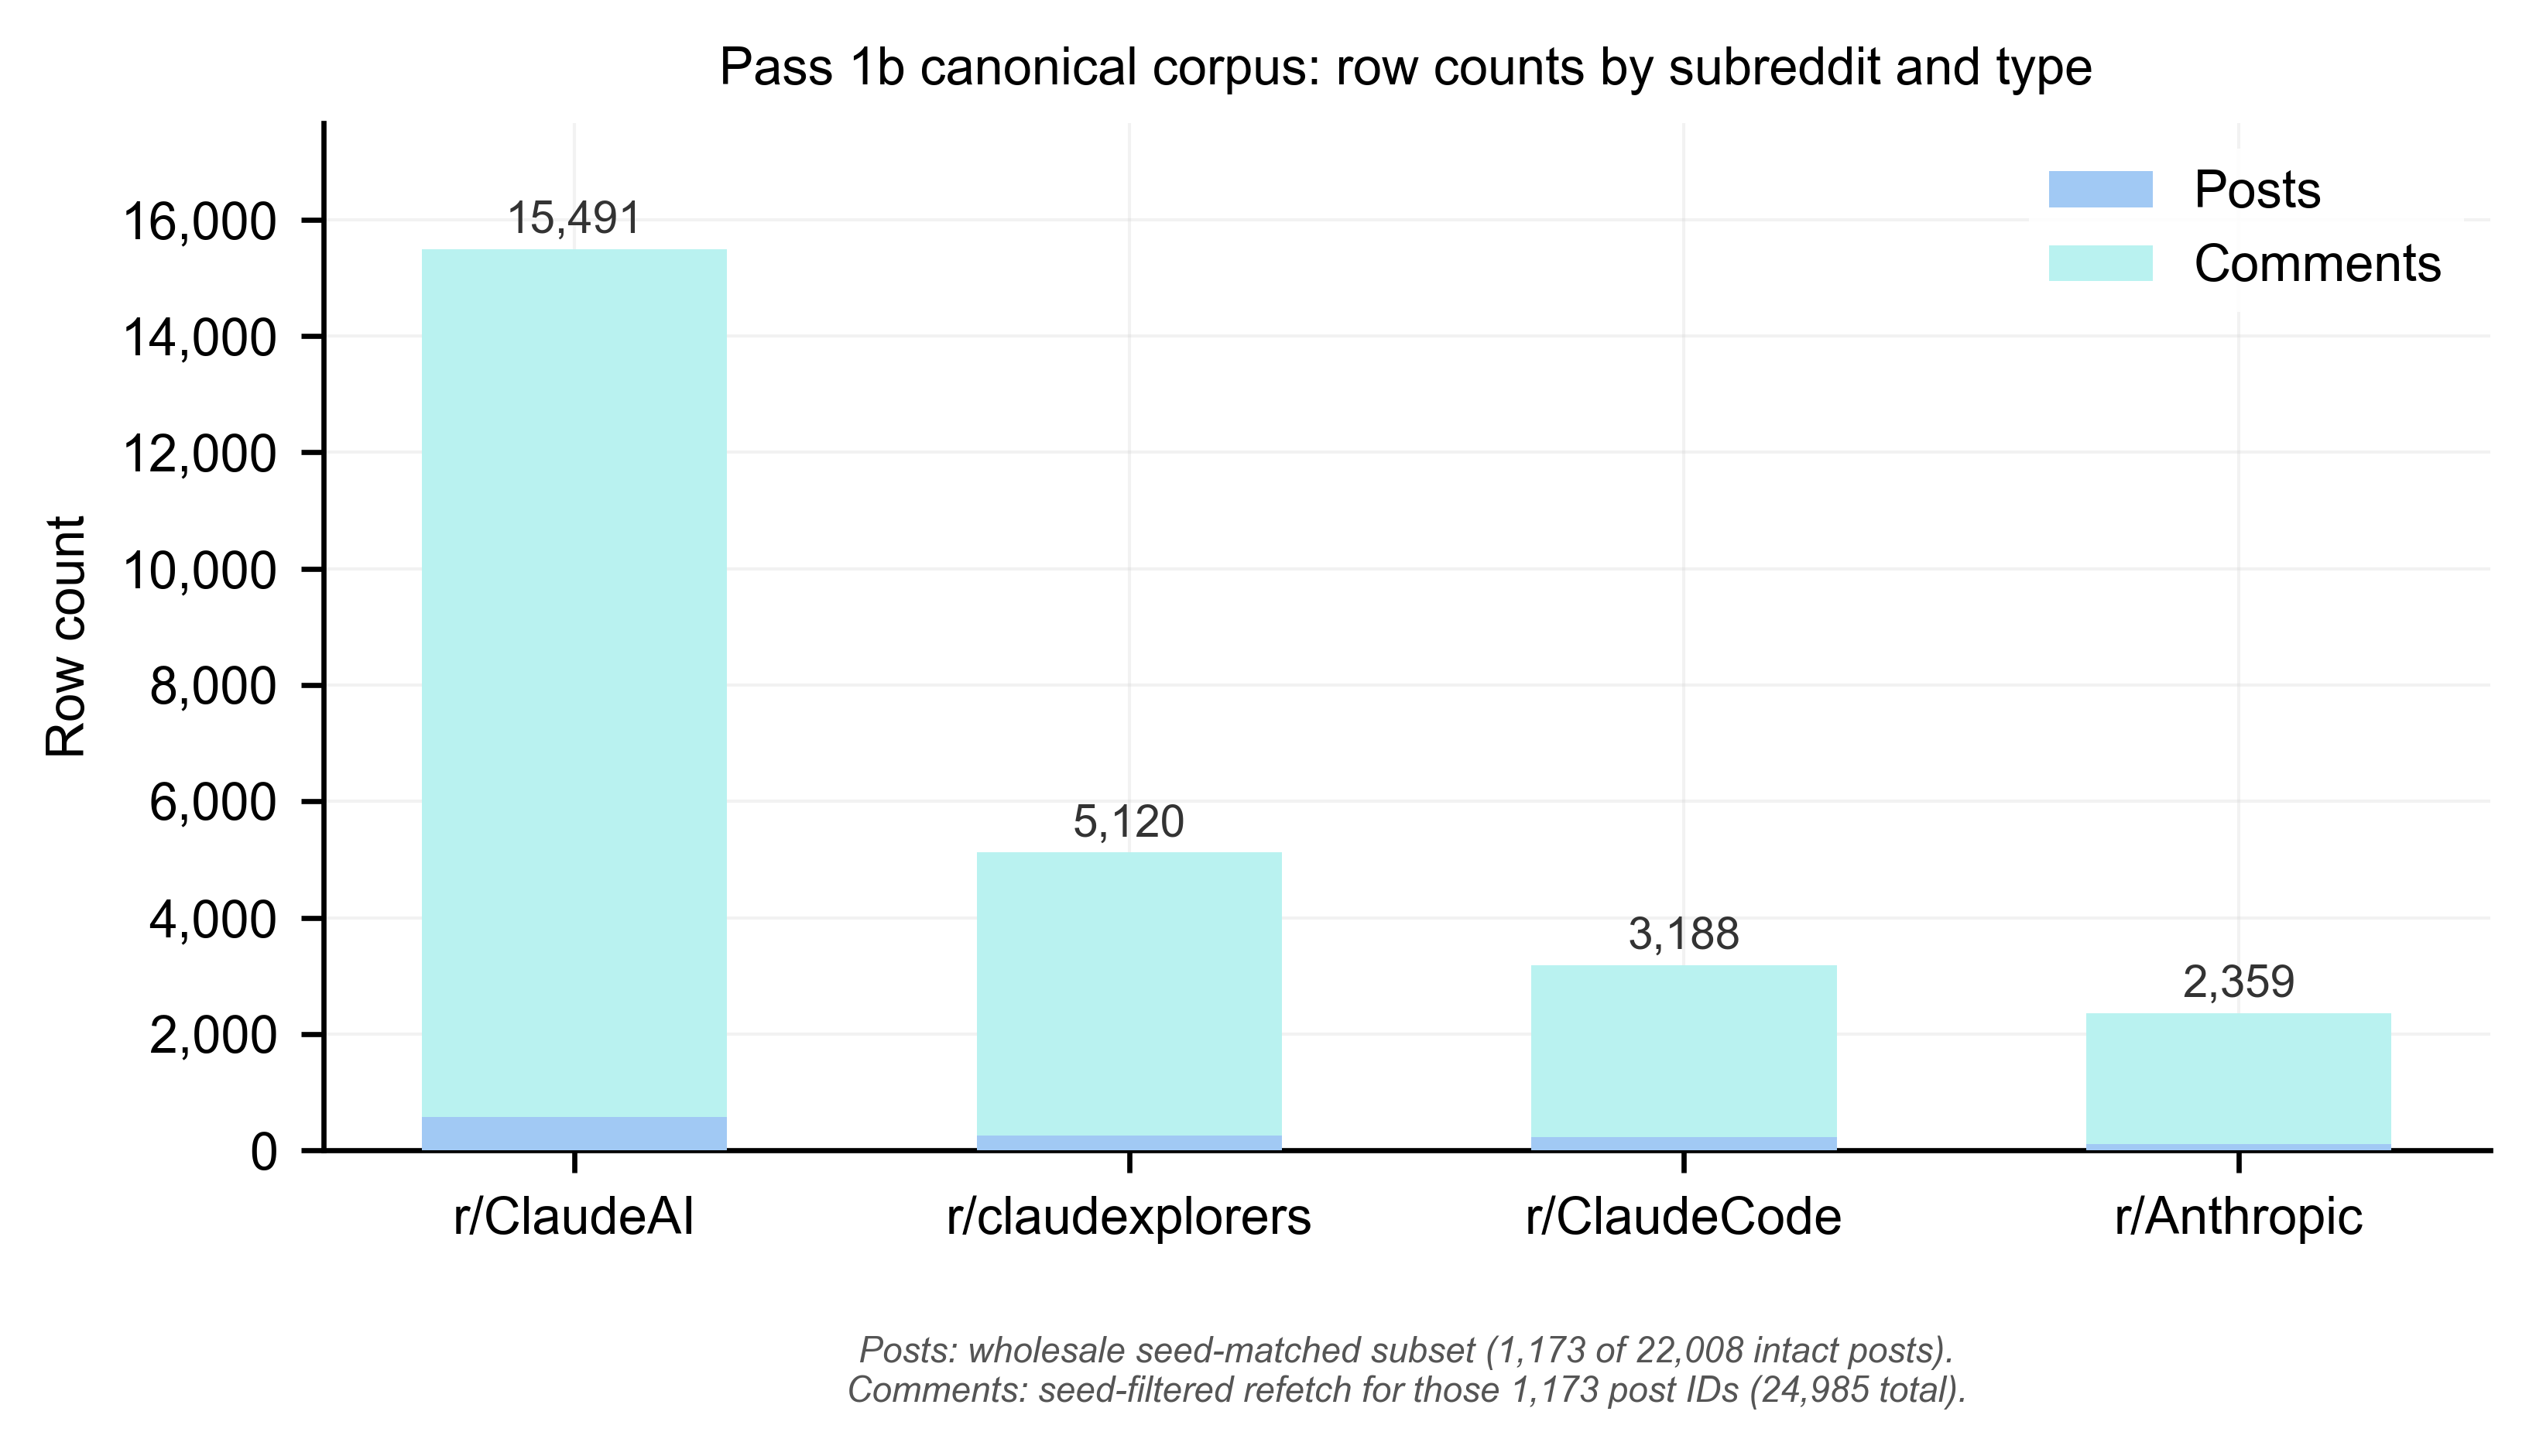
\includegraphics[width=\linewidth]{figures/corpus_composition.png}

\vspace{0.5em}
\raggedright
\textit{Note.} Pass 1b canonical corpus composition (26,158 rows total). Posts ($n = 1,173$) are a seed-term-matched subset of the wholesale August-to-December 2025 pull; comments ($n = 24,985$) are the seed-filtered refetch for those 1,173 post identifiers. r/ClaudeAI contributes the largest total (15,491 rows, 59.2\%); r/claudexplorers, the smallest community by post volume, contributes 5,120 rows (19.6\%).
\end{figure}

\subsection*{A.5 Preprocessing and quantitative-descriptive analyses}

Preprocessing follows project-standard methods-library defaults, with corpus-specific adjustments motivated by artifacts surfaced during Phase 2 frequency exploration. URL fragments are stripped before tokenization to resolve the \texttt{preview.redd.it} image-embed artifact that dominated raw bigram and trigram tables in Pass 1a; Reddit AutoModerator boilerplate is filtered as a domain stop-phrase, since the moderation string \emph{``I am a bot, and this action was performed automatically''} and its sub-n-grams occupied rank-1 trigram positions across multiple subreddits before filtering; tokens are restricted to alpha-only characters, lowercased, and constrained to a minimum length of three characters; and collocation pointwise-mutual-information computations apply a minimum co-occurrence floor of five token pairs to suppress hapax-driven inflation. Lemmatization and stop-word handling are run in four ablation variants across the cross of on/off settings per the methods-library standard, and the stops-on lemma-on configuration is reported as the primary in the prose throughout, with the remaining variants preserved in the project deliverables for readers who wish to inspect the sensitivity of the descriptive patterns to preprocessing choices. Frequency, collocation, keyword-in-context, and n-gram analyses were applied to the Pass 1b canonical corpus as descriptive-engagement instruments rather than as inferential tests, in keeping with the phenomenological posture established in Section 2.3, and the analyses were stratified along four dimensions in order to test whether the LCR-discussion vocabulary was distributed uniformly across the corpus or concentrated within identifiable substrata (row type, subreddit, Round 2 augmented seed-term match status, and release-window indicator).

\subsection*{A.6 Ethics and data handling}

All data analyzed in this paper are public Reddit posts and comments collected via the Arctic Shift academic preservation archive for non-commercial research purposes. No personally identifying information was collected, retained, or linked in the corpus, usernames were not analyzed at any stage of the pipeline, and the analyses operate on the textual content of posts and comments rather than on any user-level identifier. Brief diagnostic excerpts appear in the paper where evidentiary necessity requires the reader to see the actual model utterance or user account that grounds a structural claim, and the excerpts are presented in the form used by the original posters in their public Reddit accounts. The intent of this study, including its critical posture toward Anthropic and the LCR injection, is one that the original posters would plausibly consent to, on the grounds that the analysis serves the interests of the user community whose experiences are documented and whose published accounts of the LCR phenomenon motivated the line of inquiry pursued here.

\subsection*{A.7 Retired prior framing: the lexicon-detection approach and its precision shortfall}

An earlier iteration of this analysis operationalized the LCR phenomenon through a four-category lexicon (psychiatric attribution, help directive, concern framing, soft directive) and reported a within-corpus payload-detection rate as a headline empirical finding. The earlier framing was retired on the basis of a hand-coded validation pass in which 118 lexicon-positive cases were evaluated against a nine-dimension structural schema, returning fourteen confirmed role-violations, seven borderline determinations, and ninety-seven non-violations. The lexicon's true-positive rate against the hand-coded ground truth was 14/118, or 11.9\%. A lexicon at that level of precision cannot support inferential analyses (pointwise-mutual-information rankings, segmented regression, classifier training) without those analyses inheriting the lexicon's misspecification. The structural-signature approach reported here retires that approach in favor of two coordinated moves. Targeted retrieval with documented sampling-frame disclosure replaces wholesale lexicon-based detection: the iterative seed-term refinement of Appendix A.1 surfaces high-precision retrieval anchors (verbatim system-prompt phrasals, sample-validated reaction terms) that retrieve mechanism-discussion content rather than scoring posts for symptom presence. Phenomenological case characterization replaces prevalence estimation as the empirical centerpiece: the five-property structural signature is coded by hand against a positive-case sample, and the structural pattern is reported as a clinical-phenomenological finding rather than as a population rate. Four methodological lessons fall out of the retirement and are documented here as contributions in their own right: targeted retrieval with explicit sampling-frame disclosure is the appropriate response when phenomenon-relevant content is uncommon in untargeted Reddit discourse; row-level voice segmentation under-counts in community-reported LLM-behavior corpora and the two-tier evidence structure of Appendix A.2 is the appropriate epistemic accommodation; lexicon precision must clear a hand-coded threshold of approximately 0.85 before feeding inferential analyses, since a lexicon at lower precision trains classifiers and produces collocation rankings whose outputs inherit the lexicon's misspecification; and deterministic retrieval anchors and validated detectors must be reported as functionally distinct categories, since a phrasal lifted verbatim from corpus material recovers itself by construction and any precision figure computed against that corpus is tautological rather than evidential.

\end{document}
